% -*- Mode:TeX -*-

%% IMPORTANT: The official thesis specifications are available at:
%%            http://libraries.mit.edu/archives/thesis-specs/
%%
%%            Please verify your thesis' formatting and copyright
%%            assignment before submission.  If you notice any
%%            discrepancies between these templates and the 
%%            MIT Libraries' specs, please let us know
%%            by e-mailing thesis@mit.edu

%% The documentclass options along with the pagestyle can be used to generate
%% a technical report, a draft copy, or a regular thesis.  You may need to
%% re-specify the pagestyle after you \include  cover.tex.  For more
%% information, see the first few lines of mitthesis.cls. 

%\documentclass[12pt,vi,twoside]{mitthesis}
%%
%%  If you want your thesis copyright to you instead of MIT, use the
%%  ``vi'' option, as above.
%%
%\documentclass[12pt,twoside,leftblank]{mitthesis}
%%
%% If you want blank pages before new chapters to be labelled ``This
%% Page Intentionally Left Blank'', use the ``leftblank'' option, as
%% above. 

\documentclass[12pt,twoside]{mitthesis}
\usepackage{lgrind}
\usepackage{graphicx}
\usepackage{subcaption}
\usepackage{keyval}
\graphicspath{ {images/} }
\pagestyle{plain}

%% This bit allows you to either specify only the files which you wish to
%% process, or `all' to process all files which you \include.
%% Krishna Sethuraman (1990).
%
%\typein [\files]{Enter file names to process, (chap1,chap2 ...), or `all' to process all files:}
%\def\all{all}
%\ifx\files\all \typeout{Including all files.} \else \typeout{Including only \files.} \includeonly{\files} \fi

\begin{document}
\pagenumbering{gobble}
% NOTE:
% These templates make an effort to conform to the MIT Thesis specifications,
% however the specifications can change.  We recommend that you verify the
% layout of your title page with your thesis advisor and/or the MIT 
% Libraries before printing your final copy.

%-----------University header----------
    \begin{figure}  
        \begin{subfigure}[b]{0.3\textwidth}
            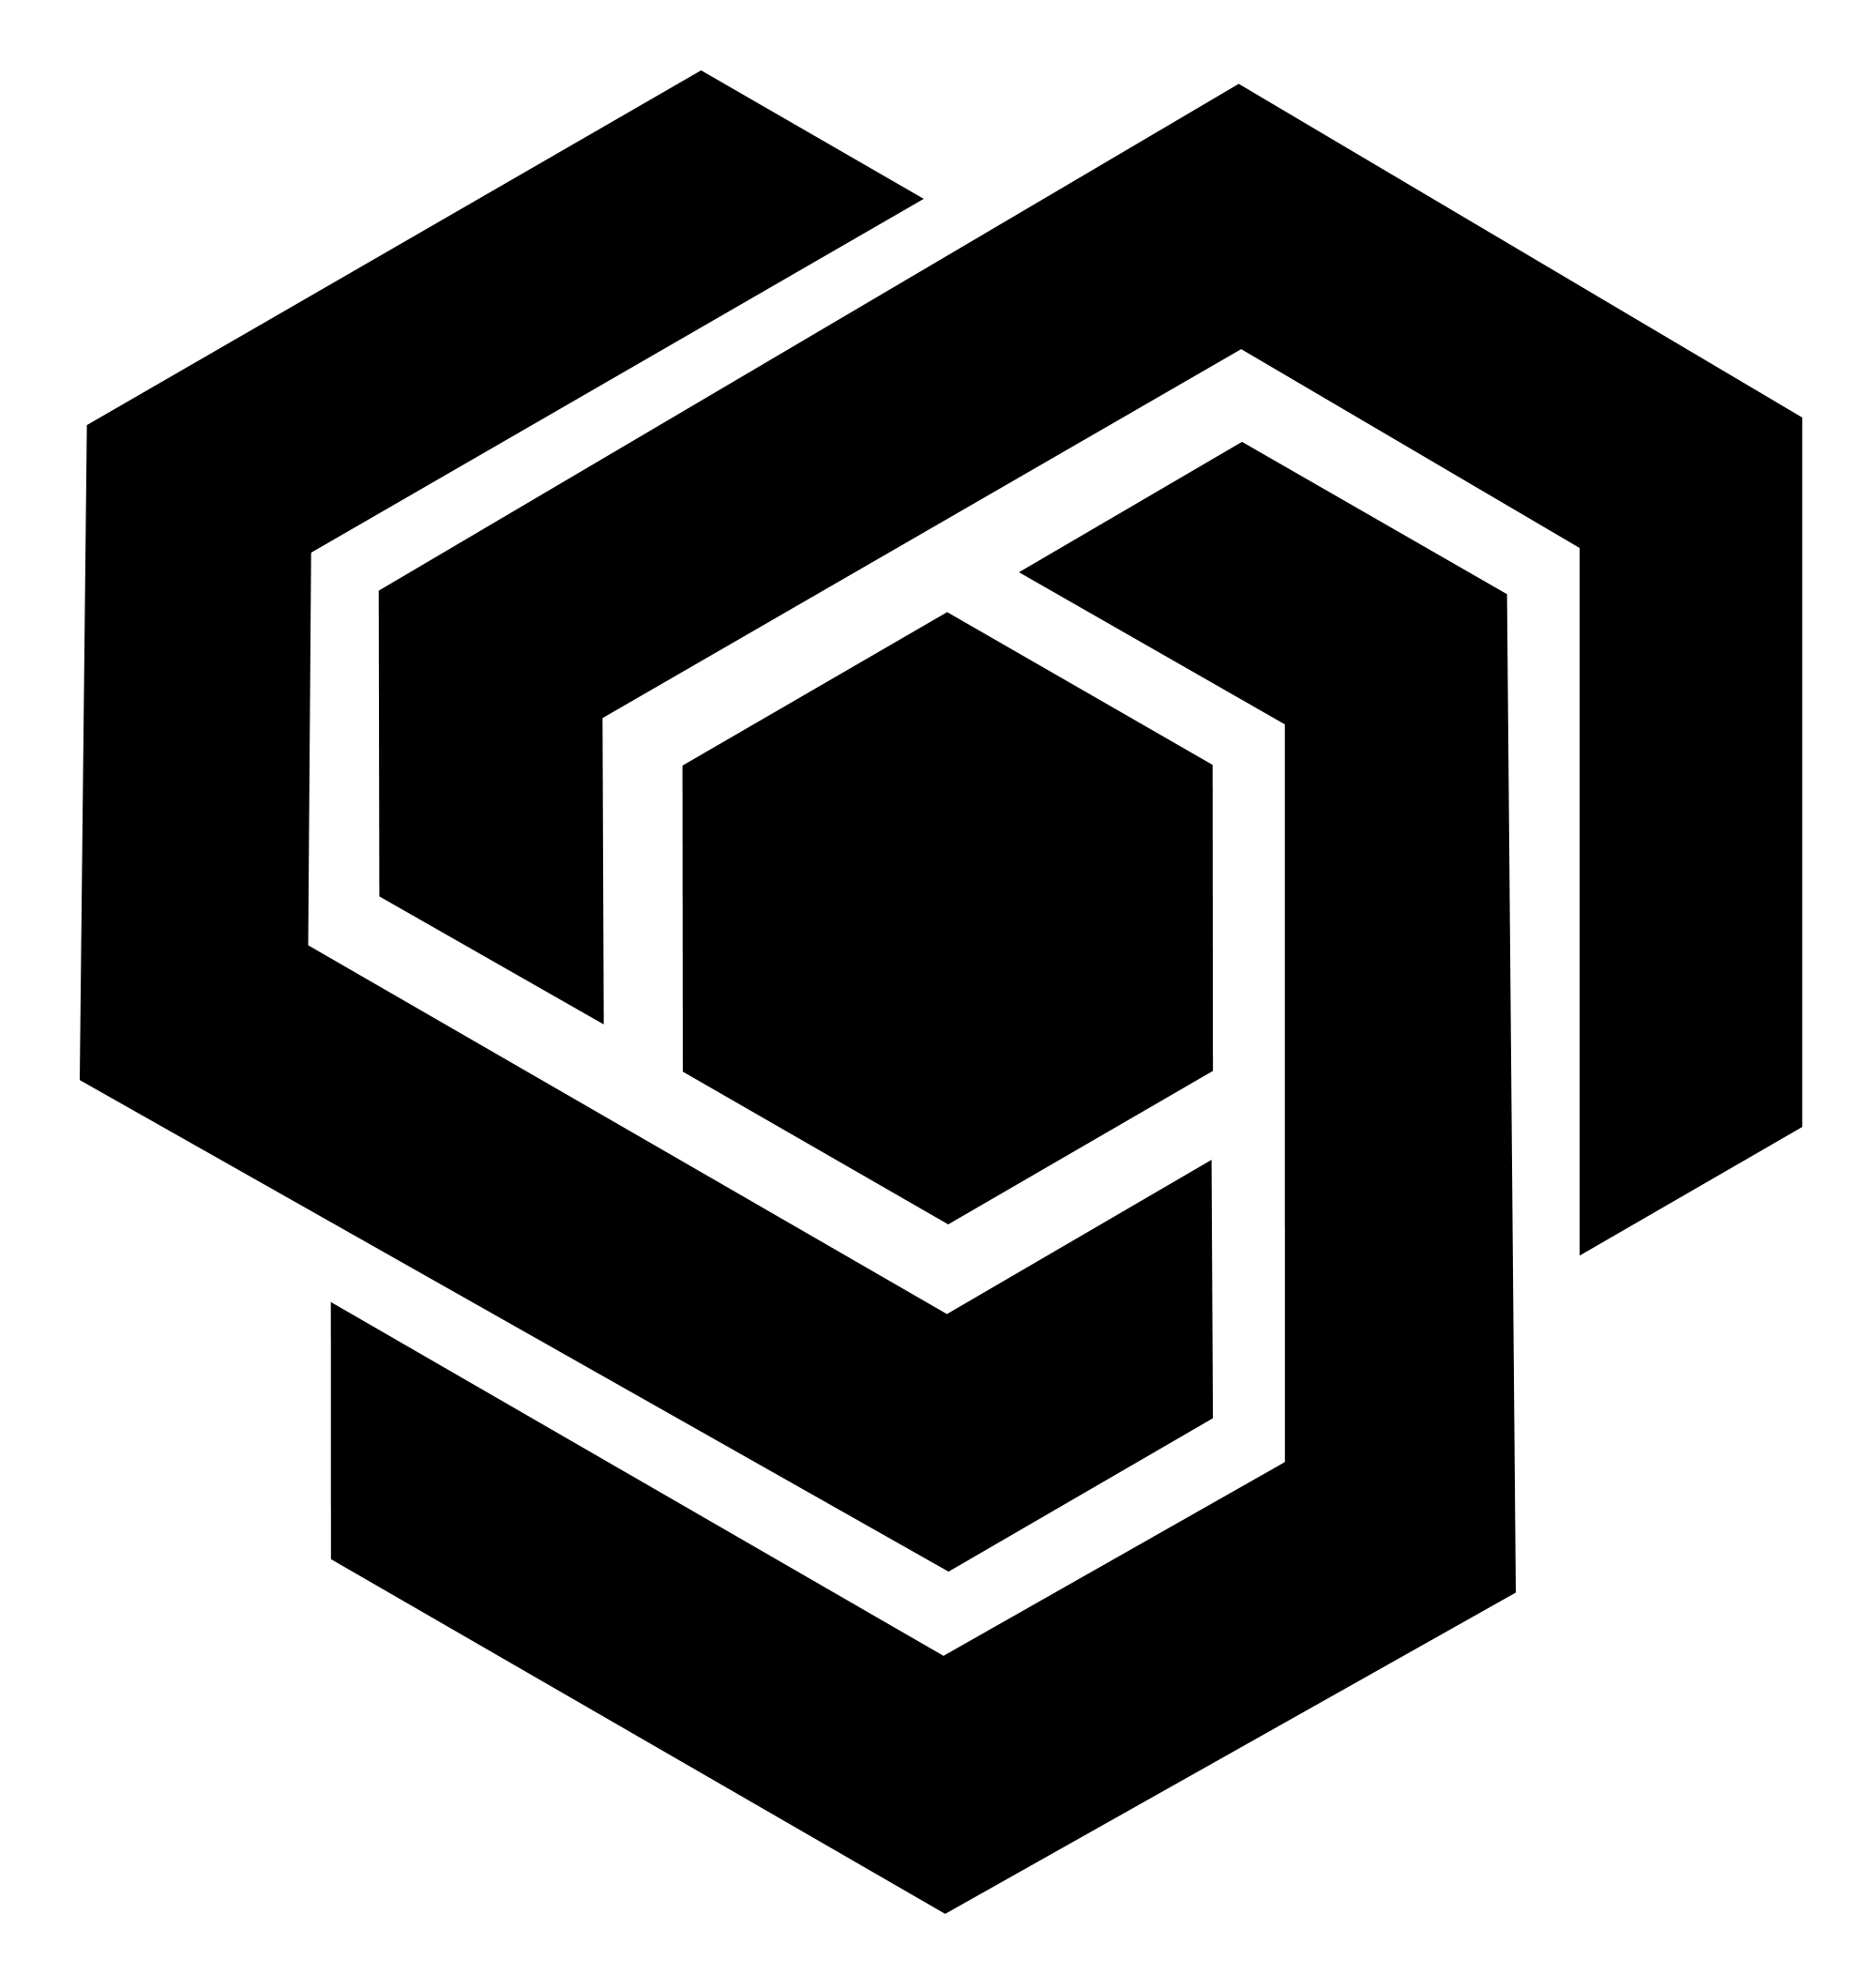
\includegraphics[width=3.5cm, left]{tu-sofia-logo.png}
        \end{subfigure}
        \begin{subfigure}[b]{0.36\textwidth}
            \centering
            \Large{Technical University Sofia}
        \end{subfigure}
        %
        % \hspace{7cm}
        %
        \begin{subfigure}[b]{0.3\textwidth}
            
\includegraphics[width=4cm, right]{fdiba-logo.png}
        \end{subfigure}
    \end{figure}
    \begin{center}
        \textbf{\large{Department of German Engineering and Industrial Management}}
        
        \vspace*{4cm}
        
        \textbf{\Huge{Integration of Semantic Technologies in the Processing of News}}
    
        \vspace{1.5cm}

        \textbf{\large{Tsvetan Dimitrov}}
        
        \vspace{1.5cm}
        
        \textbf{\large{Supervisor: Assoc. Prof. Adelina Aleksieva}}

        
        \vfill
        
        A thesis presented for the degree of\\
        Bachelor of Informatics
        
        \vspace{0.8cm}
        
        \includegraphics[width=0.4\textwidth]{university}
    
        Sofia, Bulgaria\\
        July 15, 2016
    \end{center}
% -----------University header----------

% % The abstractpage environment sets up everything on the page except
% % the text itself.  The title and other header material are put at the
% % top of the page, and the supervisors are listed at the bottom.  A
% % new page is begun both before and after.  Of course, an abstract may
% % be more than one page itself.  If you need more control over the
% % format of the page, you can use the abstract environment, which puts
% % the word "Abstract" at the beginning and single spaces its text.

% %% You can either \input (*not* \include) your abstract file, or you can put
% %% the text of the abstract directly between the \begin{abstractpage} and
% %% \end{abstractpage} commands.

% % First copy: start a new page, and save the page number.
% \cleardoublepage
% % Uncomment the next line if you do NOT want a page number on your
% % abstract and acknowledgments pages.
% % \pagestyle{empty}
% \setcounter{savepage}{\thepage}
% \begin{abstractpage}
% %% The text of your abstract and nothing else (other than comments) goes here.
%% It will be single-spaced and the rest of the text that is supposed to go on
%% the abstract page will be generated by the abstractpage environment.  This
%% file should be \input (not \include 'd) from cover.tex.

The purpose of this thesis is to develop analysis and visualisations of the news data from a public Ontotext service called News On the Web (NOW) using semantic technologies, standards of the Semantic Web and Linked Open Data. More specific tasks are generating a "News Map of Today's news" and recommending linked news and objects based on analyzing "hidden champions". Hidden champions are concepts which are not directly mentioned in the news, but are linked in the graph with a few concepts which are. For the purpose a cognitive technique called "priming" is used in which the popularity of the mentioned concepts is being spread out across the knowledge graph, following the principle of spreading activation in neural networks. The News Map will be visualised in the form of a word cloud in various options: direct popularity of the concepts based on mentions count in the news and degree of importance of these news, relative popularity - where the popularity within the current day is normalized against the popularity within the last year, concepts that are "hidden champions" and a combination of "hidden champions" and relative popularity. Analogous maps will be created for a separate news as a way to visualise the important subjects in it.
% \end{abstractpage}

% Additional copy: start a new page, and reset the page number.  This way,
% the second copy of the abstract is not counted as separate pages.
% Uncomment the next 6 lines if you need two copies of the abstract
% page.
\setcounter{page}{\thesavepage}
\begin{abstractpage}
\thispagestyle{empty}
%% The text of your abstract and nothing else (other than comments) goes here.
%% It will be single-spaced and the rest of the text that is supposed to go on
%% the abstract page will be generated by the abstractpage environment.  This
%% file should be \input (not \include 'd) from cover.tex.

The purpose of this thesis is to develop analysis and visualisations of the news data from a public Ontotext service called News On the Web (NOW) using semantic technologies, standards of the Semantic Web and Linked Open Data. More specific tasks are generating a "News Map of Today's news" and recommending linked news and objects based on analyzing "hidden champions". Hidden champions are concepts which are not directly mentioned in the news, but are linked in the graph with a few concepts which are. For the purpose a cognitive technique called "priming" is used in which the popularity of the mentioned concepts is being spread out across the knowledge graph, following the principle of spreading activation in neural networks. The News Map will be visualised in the form of a word cloud in various options: direct popularity of the concepts based on mentions count in the news and degree of importance of these news, relative popularity - where the popularity within the current day is normalized against the popularity within the last year, concepts that are "hidden champions" and a combination of "hidden champions" and relative popularity. Analogous maps will be created for a separate news as a way to visualise the important subjects in it.
\end{abstractpage}

\cleardoublepage

\section*{Acknowledgments}
I would like to thank my supervisor Assoc. Prof. Adelina Aleksieva for the guidance throughout the process of writing this thesis and the valuable feedback I received from her. I would also like to thank my other supervisor from Ontotext Milena Yankova, Ph.D and the CEO of Ontotext Atanas Kiryakov for the creative ideas and also their help in the data set work of cleaning and mapping to other Linked Open Data data sets. And last but not least I am very grateful to all my colleagues from Ontotext for their year long work and expertise in the areas of semantic technologies and text mining with whom without this thesis would not have been possible.

%%%%%%%%%%%%%%%%%%%%%%%%%%%%%%%%%%%%%%%%%%%%%%%%%%%%%%%%%%%%%%%%%%%%%%
% -*-latex-*-

% Some departments (e.g. 5) require an additional signature page.  See
% signature.tex for more information and uncomment the following line if
% applicable.
% % -*- Mode:TeX -*-
%
% Some departments (e.g. Chemistry) require an additional cover page
% with signatures of the thesis committee.  Please check with your
% thesis advisor or other appropriate person to determine if such a 
% page is required for your thesis.  
%
% If you choose not to use the "titlepage" environment, a \newpage
% commands, and several \vspace{\fill} commands may be necessary to
% achieve the required spacing.  The \signature command is defined in
% the "mitthesis" class
%
% The following sample appears courtesy of Ben Kaduk <kaduk@mit.edu> and
% was used in his June 2012 doctoral thesis in Chemistry. 

\begin{titlepage}
\begin{large}
This doctoral thesis has been examined by a Committee of the Department
of Chemistry as follows:

\signature{Professor Jianshu Cao}{Chairman, Thesis Committee \\
   Professor of Chemistry}

\signature{Professor Troy Van Voorhis}{Thesis Supervisor \\
   Associate Professor of Chemistry}

\signature{Professor Robert W. Field}{Member, Thesis Committee \\
   Haslam and Dewey Professor of Chemistry}
\end{large}
\end{titlepage}


\pagestyle{plain}
  % -*- Mode:TeX -*-
%% This file simply contains the commands that actually generate the table of
%% contents and lists of figures and tables.  You can omit any or all of
%% these files by simply taking out the appropriate command.  For more
%% information on these files, see appendix C.3.3 of the LaTeX manual. 
\tableofcontents
\newpage
\listoffigures
\newpage
\listoftables



\pagenumbering{arabic}
%% This is an example first chapter.  You should put chapter/appendix that you
%% write into a separate file, and add a line \include{yourfilename} to
%% main.tex, where `yourfilename.tex' is the name of the chapter/appendix file.
%% You can process specific files by typing their names in at the 
%% \files=
%% prompt when you run the file main.tex through LaTeX.
\chapter{Introduction}
The Semantic Web is a network of structured data represented in a format that enables automatic interpretation of its meaning. Data is represented in the form of graphs and its meaning is defined in ontologies - semantic schemes enabling automatic interpretation by deductive logical conclusion. After 2006 the Semantic Web is realized in the form of Linked Open Data - a network of data, published on different servers, but interlinked with hyperlinks (same as the hyperlinks in Web 1.0). Today there are thousands of databases (knowledge bases) published and interlinked in this way, that contain more that a trillion facts in all areas of life. Linked Data is accepted as a standard by the governments of the United States, United Kingdom and other countries for publishing public data - for example statistical information, company registers etc. Amongst the most popular databases are DBPedia (a structured version of Wikipedia) and GeoNames (containing most of Earth's geographical information).

Open Linked Data has many purposes. One of them is presenting knowledge as graphs (e.g. Google Knowledge Graph) when analyzing and indexing natural language in a process called "semantic annotation". Text is being analyzed with the purpose of finding mentions of people, companies, places and other concepts - known or unknown. Ontotext offers a solution of this kind called "Dynamic Semantic Publishing (DSP)", which persists the text, enriched with semantic tags, alongside with the knowledge graphs in a semantic graph database. Using these technologies a demo platform called "News On the Web (NOW)" has been developed, which offers browsing news, data linked with them or other news. NOW operates on a stream of about 10 000 news a month which it analyzes and links with a knowledge graph that includes DBPedia and GeoNames.

\section{Limitations of current search technologies}
Searching information on the World Wide Web is an idea dating from its very beginning. Although based on the same technologies as general information retrieval, the web brings additional challenges such as how to scale efficiently and how to implement correct ranking in its ever changing environment. Different search engines return different search results due to the variation in indexing and search processing. Google, Yahoo and Bing handle queries after processing keywords. They only search recent information given on a web page. They are constantly improving and delivering more and more accurate results, but at the end they cannot answer you a question with an aggregated result and cannot suggest you search queries which are semantically interlinked based on concepts and not only on stems and other similar keywords. 

The current web is the biggest global database that lacks the existence of a semantic structure and hence makes it difficult for a machine to understand the information provided by the user. This leads to formulating the two biggest challenges in web search: 

\begin{itemize}
    \item How can a search engine map a query to a document and retrieve meaningful information from it?
    \item The query results produced by search engines are distributed across different documents that may be connected with hyperlinks. How does the search engine efficiently recognize such distributed results? 
\end{itemize}
The Semantic Web could solve the first problem by using semantic annotations to produce structured by meaning information. The second problem could be addressed by having graph-based query models. Such a goal poses challenges of its own in the areas of 
knowledge representation, natural language processing and graph databases.

\section{Why do we need more insight?}

In today's world everything is information. The average connected consumer has access to an insane amount of it, thanks to the ubiquity of smartphone access to the web. From checking restaurant reviews and stock prices, to taking pictures of a new pair of jeans and asking the opinion of friends on Facebook, today's consumer is no longer restricted to choosing a brand through a push marketing approach. This change of direction in the purchase cycle has resulted in brands trying to better know the consumer in order to present him with the appropriate content for the purpose of advertising or just offering better customer experience. Although today buzzwords such as "Big Data" seem to be very trendy and loved by marketers the reality is that we need better insights, not more data. The data is out there and there is plenty of it easily accessible through the web. The biggest problem is that it is hard to reason about it in order to gain significant benefits. The grand vision of the Semantic Web wants to accomplish exactly that:
\begin{itemize}
    \item Enrich open data with its own semantics.
    \item Interlink those semantics between different entities and facts.
    \item Set a standardized way to access data, its semantics and other links leading to other related pieces of data.
\end{itemize}
When such knowledge is freely and easily available, a lot of cool applications become possible, e.g. content and user based recommendation systems become way more accurate if they can take advantage of user activity data and content metadata being in a unified data model and interlinked one another to find interesting patterns of user preferences towards particular content. Search becomes smarter because it indexes contextual information, rather than only keywords, and can infer related concepts. This could be extremely helpful when dealing with, e.g. news data (relating people, organisations, locations, etc.) or life sciences data (relating drugs, diseases, treatments, symptoms, etc.). To even further boost the benefits of such enriched data, machine learning techniques could be applied to train models on top of core data semantics and relations in order to predict behaviour even more accurate than when only using raw data and manually choosing and structuring its features to train upon. 

Getting more insight about the world around us and the information we produce every single day plays a huge role in our modern lives and will continue to be even more important in the future.

\section{Thesis Overview}
The aim of this thesis is to present a practical example of an intelligent application for understanding news without reading the articles themselves, based upon the Semantic Web technology stack, and to demonstrate how unstructured content could be processed into something that enables automatic reasoning of its meaning. News are a great example of a raw data source which is rich on facts and knowledge, concerning most areas of life, scattered in free text. The solution to this problem will be a pipeline which will extract the important information from free text, convert it to an RDF (Resource Description Framework) format, interlink it with other Linked Open Data data sets, import the whole data into a semantic database, called a triplestore, run interesting SPARQL queries against it to pick up trends in popularity of certain entities and finally visualise those trends and entities into a word cloud form, based on different popularity criteria and a geographic heat map of news mentioning countries all around the world. 


% \cite{ellis:bulldog,pet87,coutant:precision-compilers}.  
% \ref{ch1:opts}.
% \footnote{A description of
% the floating point format used is shown in figures~\ref{exponent-format}
%\ref{mantissa-format}.}.





\chapter{Background}
\label{chap:background}
\section{The World Wide Web}
The World Wide Web is the greatest repository of information ever assembled by
man. It contains knowledge in the form of documents and multimedia resources concerning almost every area or subject regarding our lives. All this data is freely accessible to anyone with an Internet connection. It’s success is largely due to its decentralized design and nature. Web pages are hosted by different computers and each document can point to other documents independent of where the other document is physically located. As a result everybody all over the world can publish content on the web, allowing it to grow exponentially as more and more people learn how to use it.

However the huge scale of the web leads to some consequences. Due to the sheer volume of available information, it is becoming increasingly difficult to locate useful
information. Although search engines, e.g Google, Yahoo, Bing,  can provide some assistance, they are far from perfect. For many users, locating the "right" document is still like trying to find a needle in a haystack.

\subsection{Development of the Web}
In 1990 Tim Berners-Lee developed the first version of his World Wide Web
program at CERN. The concept behind his invention was to use hypertext as a means of organizing a distributed document system. The term \textit{hypertext} refers to a collection of documents with references to each other (links) that enable readers to navigate from one document to the other without following a sequential pattern. In order to make it work on the Internet, Berners-Lee had to develop three crucial parts of the whole system:
\begin{enumerate}
    \item Mechanism for addressing documents on different machines.
    \item Protocol that allowed computers to request documents.
    \item Simple language to describe the documents.
\end{enumerate}
 Before inventing the World Wide Web there were more powerful hypertext systems available, but he built his according to simple specifications that he later published as standards. That enabled other people to use his system in their own web servers, web browsers and especially integrate them in their own websites. In time his system proved to be the most popular and most used in the world and that is why he founded W3C (World Wide Web Consortium) in order to oversee these standards and evolve them in the future.

\subsection{Enabling Technologies}
\subsubsection{HTTP}
Hypertext Transfer Protocol (HTTP) is a method for encoding and transporting information between a client (e.g. a web browser) and a web server. HTTP is the primary protocol for transmission of information across the Internet. Information is exchanged between clients and servers in the form of hypertext documents, from which HTTP gets its name. Hypertext is structured text that uses logical links (hyperlinks), between nodes containing text. Hypertext documents can be manipulated using the Hypertext Markup Language (HTML). Using HTTP and HTML clients can request different kinds of content (such as text, images, video, and application data) from web and application servers that host the content.

HTTP follows a request-response paradigm in which the client makes a request and the server issues a response that includes not only the requested content, but also relevant status information about the request in the form of \textit{headers}. This self-contained design allows for the distributed nature of the Internet, where a request or response might pass through many intermediate routers and proxy servers. It also allows intermediary servers to perform value-added functions such as load balancing, caching, encryption, and compression. HTTP resources such as web servers are identified across the Internet using unique identifiers known as Uniform Resource Locators (URLs). HTTP is an application layer protocol and relies on an underlying network-level protocol such as Transmission Control Protocol (TCP) to function.

\subsubsection{HTML}
HTML is a markup language designed for the web as a way to structure documents semantically. Web browsers can read HTML files and render them into visible or audible web pages. Internally HTML describes a hierarchical structure depicted from the ability to nest tags within each other. This structure is called the Document Object Model (DOM) and plays an important role when manipulating HTML with Javascript for achieving web page interactivity. HTML5 is the newest standard which adds many new features to the language such as native support for including and handling multimedia and graphical content - the new \verb|<video>|, \verb|<audio>| and \verb|<canvas>| elements, support for Scalable Vector Graphics (SVG) content and MathML for mathematical formulas. Another neat feature are semantic tags used to enrich the semantic content of documents, new page structure elements such as \verb|<main>, <section>, <article>, <header>, <footer>, <aside>, <nav>| and \verb|<figure>| are added.  

\subsubsection{CSS}
Cascading Style Sheets (CSS) is a style sheet language used for describing the presentation of a document written in a markup language. CSS is designed primarily to enable the separation of document content from document presentation, including aspects such as the layout, colors, and fonts. This separation can improve content accessibility, provide more flexibility and control in the specification of presentation characteristics, enable multiple HTML pages to share formatting by specifying the relevant CSS in a separate .css file, and reduce complexity and repetition in the structural content.

\subsubsection{Javascript}

Javascript is a dynamic programming language originally designed for the web and standardized in the \textit{ECMAScript} language specification. It is a multi-paradigm language, supporting imperative, object-oriented and functional programming. Functions are treated as first class citizens. A lot of language constructs are inspired by languages such as Java and Scheme. Although meant to live in the browser, Javascript has proven over time to be suitable as a general-purpose programming language. NodeJS is an example of a runtime environment allowing to use Javascript for server side development, MongoDB accepts queries written in Javascript, Adobe's Acrobat and Adobe Reader support JavaScript in PDF files etc..

\section{Knowledge Representation}
Knowledge Representation is a field of artificial intelligence that deals with the symbolic representation of knowledge of a subject area. This is accomplished in an automatic way by using reasoning programs. More informally, it is a part of AI, which is concerned with thinking and how thinking leads to intelligent behavior. As a field of study, it proposes an approach to understanding Intelligent behavior that is radically different from the others. Instead of studying people or animals (their biology, their nervous system, their psychology, their sociology, their development, etc.), it is the people's knowledge that is to be studied. It is accepted that people possess the right knowledge and this knowledge can apply in different situations in order to achieve their goals. Therefore, in the range of KR you deal with knowledge and not with the owner of knowledge.

The goal is the development of formalism by which knowledge about the world can be described in an abstract way and can be effectively used to implement intelligent applications. The nature of knowledge is a difficult (philosophical) question. KR is only limited to conceptual knowledge. Other types of knowledge are temporal knowledge, spatial knowledge, procedural knowledge, knowledge of knowledge, etc. KR makes a description of the concept of a lecture, a computer, an illness, a workpiece, etc. - a "what is a XYZ" description.

\subsection{Logic in Knowledge Representation}
The main goal of logic (there is no uniform study of logic but many) is to express knowledge about a certain phenomena or a specific part of the world by means of a formal language. The core that defines reasoning about real world things is their encoding by using a precise set of deterministic rules called \textit{inference rules}, that everyone agrees upon. Correct reasoning enables particular knowledge to be represented by a logical sequence from a set of facts. In logic correct reasoning chains are constructed by chaining applications of simple inference rules that transform the original knowledge in a derived conclusion. 

\subsubsection{First Order Logic}
First Order Logic is a formalism by which one can describe statements very expressively. Just like prepositional logic, first order logic has:

\begin{itemize}
    \item a syntax that determines which strings are its valid formulas.
    \item semantics that determines the meaning of each of these formulas.
\end{itemize}

FOL deals with objects (for example, the residents of Frankfurt and their relationships or the natural numbers and their addition and multiplication) and statements about their properties. In contrast, the propositional logic deals not with objects but only with "true" and "false" statements and their combination.
The world is modeled on terms of:

\begin{itemize}
    \item \textit{Objects} - things with individial identities.
    \item \textit{Features} - characteristics of objects that distinguish an object from other objects.
    \item \textit{Relations} - connections between sets of objects.
    \item \textit{Functions} - a subset of relations, which only take one value as input.
\end{itemize}

FOL overtakes, modifies and extends the syntax of prepositional logic:
\begin{itemize}
    \item Similarities:
    \begin{itemize}
        \item Operators $\neg, \wedge, \vee, \rightarrow, \leftrightarrow$.
    \end{itemize}
    \item Differences:
    \begin{itemize}
        \item Variables do not correspond to “true” oder “false” expressions, but to elements of the universe of a  $\sigma$-structure.
        \item Variables are not atomic formulas any more.
    \end{itemize}
    \item What is new:
    \begin{itemize}
        \item Quantifiers: $\exists$ ("does exist") and $\forall$ ("for all").
        \item There are symbols for elements from the $\sigma$ signature.
    \end{itemize}
\end{itemize}
\subsubsection{Description Logic}
Description logic is a family of knowledge representation formalisms, which allow the key terms of a field to be described in a formal, logic-based language. Such types of logic are used in various applications, but especially for the semantic annotation of data in data integration and the World Wide Web. The familiar Web Ontology Language (OWL) is substantially based on a description logic. Syntax and semantics are here always well-defined logic-based:

\begin{itemize}
    \item \textit{Syntax:}  recursive definition in which the constructors that can be used to form concept terms are stated. Some constructors are related to logical constructors in first-order logic (FOL) such as \textit{intersection} or \textit{conjunction} of concepts, \textit{union} or \textit{disjunction} of concepts, \textit{negation} or \textit{complement} of concepts, \textit{universal restriction} and \textit{existential restriction}. Other constructors have no corresponding construction in FOL including restrictions on roles for example, \textit{inverse}, \textit{transitivity} and \textit{functionality}.
    \item \textit{Semantics:} strengthens the meaning of representing knowledge in a precise, unambiguous way.
    \begin{itemize}
        \item \textit{Declarative semantics:} independent from the processing, e.g. you want to represent (describe), not to program in something like Prolog. It enables widespread application independence and is based on logical structures.
    \end{itemize}
\end{itemize}
Central elements of descriptive logic are:
\begin{itemize}
    \item \textit{Concepts} - describe classes from objects.
    \begin{itemize}
        \item person, course, university, table, student, etc.
    \end{itemize}
     Can be described by using logical expressions (formulas).
    \item \textit{Roles} - binary relations between objects.
    \begin{itemize}
        \item listen, teach, partOf, etc.
    \end{itemize}
    In most cases can be described by simple expressions. 
    \item TBoxes (assertion of concepts) - define and connect concepts.
    \begin{itemize}
        \item \textit{Definition of concept}\newline 
        student $\equiv$ person $\sqcap \exists$ listens.lecture  
        \item \textit{General background knowledge / Constraint}\newline
        student $\sqcap$ lecture hall $\sqsubseteq \bot$
    \end{itemize}
    \item \textit{ABoxes (assertions of individuals)} - describe individuals (objects) and their features.
        \begin{itemize}
            \item student(hans)\newline
            lecture $\sqcap \exists$ subject.informaticsSubject(blv)\newline
            listens(hans, blv)
        \end{itemize}
\end{itemize}

\subsection{Semantic Networks and Frame Systems}
One of the oldest knowledge representation formalisms are semantic networks. Each concept in a semantic net is represented by a node in a graph. Concepts that are
semantically related are connected by arcs, which could be optionally labeled. Implication of meaning is represented by the way a concept is connected to other concepts. Special arcs are used to represent abstraction, although their semantics are often unclear. Now it is rather common to use two arcs for this purpose. An \textit{is-a} arc indicates that one concept is a subclass of another, while an \textit{instance-of} arc indicates that a concept is an example of another concept (see \textit{Figure \ref{fig:semantic_net}}). These types of arcs have correlations in basic set theory: \textit{is-a} is like the subset relation and \textit{instance-of} is like the element of that relation.
A collection of \textit{is-a} arcs specifies a partial order on classes often referred to as a \textit{taxonomy} or \textit{categorization hierarchy}. The taxonomy can be used to adjust the abstraction level - either generalize a concept to a more abstract class or specialize a class to its more specific concepts.

\begin{figure}[h!]
    \centering
    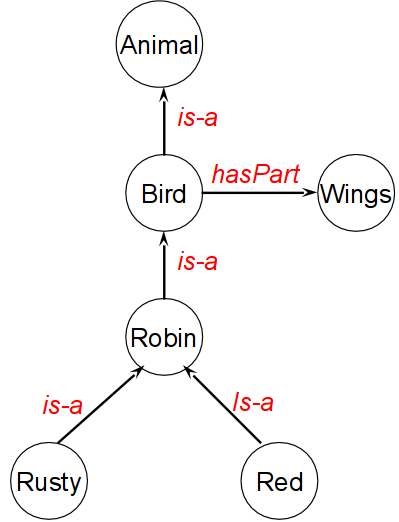
\includegraphics[width=10cm]{semantic_net}
    \caption{Semantic net inheritance}
    \label{fig:semantic_net}
\end{figure}

In the 1970's Marvin Minsky introduces frame systems. In the terminology of such systems, a frame is a named data object that has a set of slots, where each slot
represents a property or attribute of the object. Slots can have one or more values (called fillers), some of which may be pointers to other frames. Since each frame has a set of slots that represent its properties, frame systems are usually considered to be
more structured than semantic networks. However, it has been shown that frame systems are similar to semantic networks. Famous KR languages based on frame systems are KRL and KL-ONE (based on description logic). 

\subsection{Ontologies}
In order for information from different sources to be integrated, there needs to be a shared understanding of the relevant domain. Knowledge representation formalisms provide structures for organizing this knowledge, but provide no mechanisms for sharing it. Ontologies provide a common vocabulary to support the sharing and reuse of knowledge. Although there is no universally accepted definition, the main thread of ontology in the philosophical sense is the study of entities and their relationships. The question an ontology asks is: \textit{What kinds of things exist or can exist in the world, and what manner of relations can those things have to each other?}. On the Semantic Web ontologies define the concepts and relationships (also referred to as “terms”) used to describe and represent an area of concern. They are used to classify the terms that can be used in a particular application, characterize possible relationships, and define possible constraints on using those terms. An example is to use ontologies to organize knowledge. Libraries, museums, newspapers, government portals, enterprises can now use ontologies modelling their knowledge domain by using standard formalisms which aid in sharing (data integration) and leveraging the power of other interlinked open data.

\section{Semantic Web}
The Semantic Web reveals the next generation in the development of the Internet. It enables interconnectedness of data from one source to another and the representation of this data in a machine readable form. This way computers can understand the information and can process ever more demanding tasks. The Semantic Web consists of a stack of standards and best practices for sharing data and its semantics across the Internet in order to be used by applications. Heavily backed up by the W3C the Semantic Web is also built using the same type of standards such as, e.g. HTML and CSS. These standards are: the RDF data model, the SPARQL query language, the RDFS and OWL standards for vocabularies and ontologies. A product could be created with built-in semantics but if it does not adhere to these standards it cannot be part of the Semantic Web. 

\subsection{Resource Description Framework (RDF)}
The Resource Description Framework (RDF) is the result of the work of the W3 Consortium for a web infrastructure for metadata. It is standardized on 22.February 1999. It represents a data model with well-defined formal semantics, based on directed graphs and modelling data as a set of triples \textit{Triple (subject, predicate, object)}. A set of triples builds a graph.
\begin{figure}[h!]
    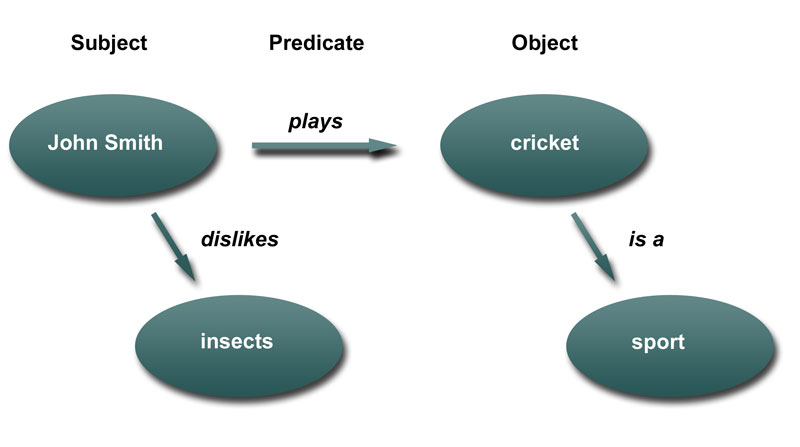
\includegraphics[width=\linewidth]{rdf-triple-example}
    \caption{RDF Triple Scheme}
    \label{fig:view}
\end{figure}

A \textit{resource} is something that is uniquely identified and can express something about it. \textit{Subjects} und \textit{predicates} are always resources and an \textit{object} could either be a resource or a \textit{literal}. Literals could be strings or other datatypes (numbers, dates, etc.).

A crucial difference in comparison to other data models such as the relational data model is that RDF represents information as a graph and all objects are connected by edges. For example the sentence "Dresden is a city in Sachsen." partitions itself as "Dresden" and "Sachsen" being objects that are connected with the edge "is a city in". In RDF the following triple is constructed: \textit{subject (Dresden)}, \textit{predicate (is a city in)} and the \textit{object (Sachsen)}. In its essense this is everything. So why bother having this model? HTML describes the structure of a web page in a standardized fashion. This leads to strong decoupling from the used browsers when consuming web page content. The answer is that the same has to be achieved from RDF, but for data.

Data from the Web today is being provided through various custom formats and interfaces. If you want to aggregate it to find it new applications, these interfaces must be individually connected and brought up in a new individual format. In addition today lots of data is listed directly in web pages, e.g. in HTML. In order to utilize this data, it must be extracted individually from the websites. This means for a very high expenditure and also restricts the actual availability of data and sometimes associates with poorer quality. All of this changes when RDF is used because it eliminates the transformation of data since it is provided and used in the same exact model.

In addition individual graphs could be connected with new links, something understood as the \textit{"Linked Data"} concept which is all about connecting information on a topic so that it could be structurally navigated.

RDF is a data model which could be represented in different formats like e.g. XML (RDF/XML), HTML (RDFa), JSON (JSON-LD) or Turtle (a lighter more human readable format). RDF itself is schema-less, but there do exist different schemes like OWL (Web Ontology Lanquage) and RDFS (RDF Schema). There is also SPARQL (SPARQL Query Language) which is a query language like SQL but for RDF.

\subsection{Web Ontology Language(OWL)}
The OWL (Web Ontology Language) is designed to enable processing of the information content of applications instead of only presenting it to the user. OWL facilitates additional vocabulary in conjunction with formal semantics and allows stronger interpretations of web content than XML, RDF and RDFS. It consists of three languages with increasing expressiveness : OWL Lite, OWL DL and OWL Full. It differs \textit{classes, properties and instances} and works according to the open world assumption which allows  inferring new facts related to a class, even though previously you had none for this class. OWL also consists of a set of axioms which describe the classes, their properties and the relationships between them.

\subsection{SPARQL Query Language (SPARQL)}
SPARQL is a query language, i.e. a semantic query language for databases storing and manipulating RDF. It is a standard which has been created by the RDF Data Access Working Group (DAWG) of the W3C and is recognized as one of the key technologies of the Semantic Web. Although SPARQL queries RDF, it is not only limited to data in the RDF formats. Commercial and open source utilities are available for handling relational data, XML, spreadsheets and other formats such as RDF, so that you can write SPARQL queries against each of these sources or a combination of them. The "protocol" part of the SPARQL standard sets rules for clients and SPARQL processing servers on how to exchange results between each other. Those rules are specified in a document separate from the query language specification and it usually concerns only developers of SPARQL-processors.

The query in the next example finds the names of all African capitals and the countries in which they are located.

\begin{verbatim}
PREFIX abc: <http://example.com/exampleOntology#>

SELECT ?capital ?country
WHERE {
    ?x abc:cityname ?capital ;
       abc:isCapitalOf ?y .
    ?y abc:countryname ?country ;
       abc:isInContinent abc:Africa .
}
\end{verbatim}

Variables are prefixed with a "?" (a possible alternative is also "\$"). As a result the query above returns all variable assignments for "?capital" and "?country", that match the four RDF-triple patterns. Writing out the whole URIs each and every time ruins the readability of the query so that is why prefixes are used. In this case "abc:" stands for \verb|"http://example.com/exampleOntology\#"|.

\subsection{Triplestores (semantic databases)}
When you want to save lots of triples, persisting them in a huge file as Turtle or RDF/XML is probably not the brightest idea, because at this scale you will need a system that indexes your data for fast retrieval when searching and also a system that decides which parts of your data to keep in memory for optimal performance without swapping to disk.
This is exactly the job of a DBMS (Database Management System), e.g. MySQL or Oracle, but one that is optimized for RDF data. Such types of databases are called triplestores. One of the best on the market today are \textit{GraphDB from Ontotext} und \textit{Virtuoso from OpenLink}.

\begin{figure}[h!]
    \caption{Famous triplestore logos}
    \begin{subfigure}[b]{0.5\textwidth}
        \centering
        
\includegraphics[width=7.5cm]{graphdb-logo}
        \caption{Ontotext GraphDB logo}
        \label{fig:view}
    \end{subfigure}
    \begin{subfigure}[b]{0.5\textwidth}
        \centering
        
\includegraphics[width=5cm]{virtuoso}
        \caption{OpenLink Virtuoso logo}
    \label{fig:view}
    \end{subfigure}
\end{figure}

\section{Linked Data}

The term \textit{Linked Data} refers to a set of best practices for publishing and connecting
structured data on the Web. These best practices have been adopted by an increasing number of data providers over the last years, leading to the creation of a global data space containing billions of facts - the \textit{Web of Data}. 

The Web today relies on HTML documents connected by untyped hyperlinks. Linked Data on the other hand needs documents containing data in RDF format. However rather than simply connecting these documents, Linked Data uses RDF to make typed statements that link arbitrary things in the world. The result is what we refer to as the
Web of Data - a network of connected data pieces (facts) that are strongly interconnected enabling easy machine processing and new types of applications based on this technology.

There is already a lot of structured data accessible on the Web through Web 2.0 APIs, e.g. the APIs from Google, Yahoo or Amazon. Compared to them, Linked Data has the advantage of providing a single, standardized access mechanism instead of relying on diverse interfaces and result formats. This gives the following capabilities regarding data sources:

\begin{itemize}
    \item Easy crawling by search engines.
    \item Access using generic data browsers.
    \item Adds links between data from different data sources.
\end{itemize}

\subsection{Linked Data Principles}
Berners-Lee (2006) outlined a set of "rules" for publishing data on the Web in a way that all
published data becomes part of a single global data space:
\begin{enumerate}
    \item Use URIs as names for things.
    \item Use HTTP URIs so that people can look up those names.
    \item When someone looks up a URI, provide useful information, using the standards
(RDF, SPARQL).
    \item Include links to other URIs, so that they can discover more things.
\end{enumerate}

These rules have become known as the \textit{"Linked Data principles"}, and provide a basic recipe for publishing and connecting data using the infrastructure of the Web while adhering to its architecture and standards.

\subsection{Linked Open Data (LOD) project}

The most popular example of adoption and application of the Linked Data principles is
the \textit{Linked Open Data} project, a big community effort that started in January
2007 and is supported by the W3C Semantic Web Education and Outreach Group. The ongoing aim of the project is to start building the Web of Data by identifying existing data sets that are available under open licenses, convert them to RDF, according to the Linked Data principles, and publish them on the Web.

The early stages of the project involved researchers and developers from universities and small companies. Since then the project has grown
considerably and large organisations such as the BBC, Thomson Reuters and the Library of Congress started contributing to the project. This growth is enabled by the open nature of the project, where anyone can participate simply by publishing a data set according to the Linked Data principles and interlinking it with existing data sets. The figures below depict the range and scale of the whole initiative: 

\begin{figure}[h!]
    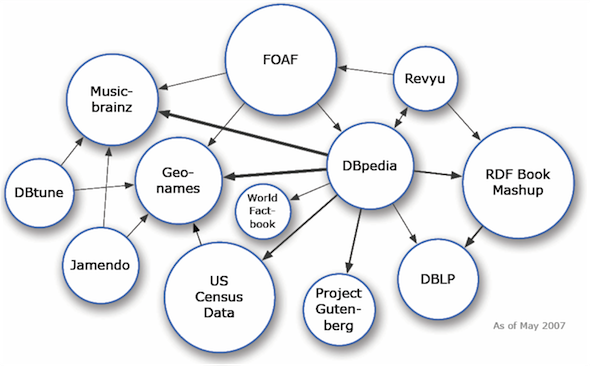
\includegraphics[width=\linewidth]{lod-cloud-may-2007}
    \caption{Linked Open Data state - May 2007}
    \label{fig:view}
\end{figure}

\begin{figure}[h!]
    \includegraphics[width=\linewidth]{lod-cloud-august-2014}
    \caption{Linked Open Data state - August 2014}
    \label{fig:view}
\end{figure}

\subsection{Publishing Linked Data on the Web}
Publishing a data set as Linked Data on the Web involves the following three basic steps:
\begin{enumerate}
    \item Assign URIs to the entities described by the data set. These entities must be retrievable (dereferenceable) from that URI over the HTTP protocol as RDF representations.
    \item Set RDF links to other data sources on the Web, so that clients can navigate the Web of
    Data as a whole by following RDF links.
    \item Provide metadata about published data, so that clients can assess the quality of published data and choose between different means of access (SPARQL endpoint, RDF dumps) besides dereferenceable URIs.
\end{enumerate}

As already stated above URIs should be valid, i.e. a request to that URI should provide the searched entity's RDF representation. Data providers can choose between two HTTP URI usage patterns to identify entities:
\begin{itemize}
    \item \textbf{303 URIs} - use a special HTTP status code, "303 See Other", to distinguish non-document resources from regular web documents. The server is configured to answer requests to such URIs with a 303 HTTP status code and a \textit{Location} header providing a new URL to a document describing the resource, e.g.:
    \begin{enumerate}
        \item Make request to \verb|http://example.com/id/alice|.
        \item Server responds with 303 status code and employs content negotiation (\verb|Accept: application/rdf+xml|, other type or none) to send either the URL of an HTML document or RDF.
        \item Requests for HTML would be redirected to \\ \verb|http://example.com/people/alice| and requests for RDF data would be redirected to \verb|http://example.com/data/alice|.
    \end{enumerate}
    \item \textbf{Hash URIs} - URIs that contain a special part called a \textit{fragment} which is usually not interpreted as part of the URI, e.g. \verb|http://example.com/data#alice|. Requesting clients will always strip off the fragment part, resulting in a request to this URI: \verb|http://example.com/data|, which will serve an RDF document describing all entities under the \verb|"data"| namespace. Again by employing content negotiation one can redirect to an HTML document \\ (\verb|http://example.com/data.html|) or other RDF descriptions \\ (\verb|http://example.com/data.rdf|).
\end{itemize}
Hash URIs have the advantage of usually making less requests in order to retrieve a whole set of RDF descriptions, but if the data set is huge and you only want to retrieve a particular description of an entity then 303 URIs are better suited due to having more fine-grained control on the server side.

In an open environment like the Web, different information providers publish data about the same real world entity like a geographic location or a person and thus introduce different URIs to identify the same entity. DBpedia uses the URI \verb|http://dbpedia.org/resource/Berlin| to identify Berlin, while Geonames uses the URI
\verb|http://sws.geonames.org/2950159/| to identify Berlin. As both URIs refer to the same thing, they are called URI aliases. URI aliases are common because it cannot be expected that all information providers agree on the same URIs to
identify an entity. URI aliases also provide an important social function to the Web of Data
as they are dereferenced to different descriptions of the same entity and allow different views and opinions to be expressed. In order to still be able to track these diverse opinions, it is a common
practice that data providers set \verb|owl:sameAs| links to all URI aliases they know about.
\chapter{Smart processing of news}
\label{chap:news-pipeline}
This chapter will present the whole news processing pipeline from raw text data to interlinked RDF with other Linked Open Data data sets. The steps will include extraction of relevant entities and relationships between them, conversion to RDF, a data preparation step that includes data cleanup and interlinking with other public RDF data sets. Finally everything will be imported in an Ontotext GraphDB\textsuperscript{TM} triplestore repository where interesting aggregating SPARQL queries will be executed against the imported metadata to find trends of popularity.

\section{Concept Extraction}
The first processing step of our whole pipeline is the extraction of relevant entities from free text, in this case news articles, and finding relationships between them. Entities are called those phrases in text that usually carry most of the meaning in a piece of information. They are divided into categories/classes of real world things, e.g. people, organisations etc.. When examining the context of the article being processed, different entities could be interlinked based on it. Those are the relationships between them which add significant information value to the discovered metadata. 

The \textit{Ontotext Concept Extraction Pipeline} is a tool for automated analysis of large volumes of textual content, through which mentions of specific concepts and relationships between them can be discovered and represented in a machine-processable format. It enriches the content aggregated from various news sources based on data from DBpedia, WikiData, GeoNames and others. The pipeline utilizes a wide variety of linguistic and algorithmic resources – such as semantic gazetteers, rules triggered by particular linguistic patterns, various statistical models for classification and sequence tagging trained against human-annotated corpora, etc.. These resources are chained together in a sequence (hence the name pipeline) that provides content enrichment of gradually increasing complexity, where each phase builds upon the results produced by the one that precedes it. The concept extraction pipeline recognises mentions of entities such as Person, Organisation, and Location, and links them if possible to a particular Knowledge Base (DBpedia, WikiData, GeoNames etc.). It also tags the particularly relevant noun phrases, called key phrases thus allowing a fast grasp into the topic of the document. Furthermore it detects relationships between the extracted entities, as well as their relevance and confidence to the text. Due to the fact that text mining and natural language processing techniques are outside the scope of this thesis, we will not examine in more details the workflow of this processing step.

\section{RDF Data Preparation}
After processing some raw news data to discover relevant mentions and converting them to RDF, the next step is to interlink NOW RDF data with other data sets that will give more information about those mentioned entities. For this purpose the following mappings and data sets are used: 
\begin{itemize}
    \item DBPedia
    \item GeoNames
    \item \verb|sameAs| statements between DBPedia and Geonames
    \item NOW RDF news data
\end{itemize}

\subsection{Data Cleanup}
In order to make everything work correctly some data cleanup is required and some additional mappings have to be introduced:
\begin{enumerate}
    \item \subsubsection {Delete dbo:subsidiary misuse linking company to country or town}
    
    \textbf{dbo:subsidiary} is erroneously used to indicate that a company has a subsidiary in a specific country or town. This implies that the company owns the country or the town so it needs to be removed. The following query fixes the most obvious problem:
    
\begin{verbatim}
PREFIX dbo: <http://dbpedia.org/ontology/>

DELETE { ?parent dbo:subsidiary ?child }
WHERE {
  ?parent dbo:subsidiary ?child.
  ?child a ?class .
  FILTER (?class IN (dbo:Town, dbo:Country))
}
\end{verbatim}

    \item \subsubsection{Additional mappings fixing messy industry classifiers}
    DBPedia's industry classifiers are very noisy. There are multiple identifiers used for one and the same syntactic variation. They are also unstructured, e.g. \textit{RailTransport} is by no means connected to \textit{Transport} and \textit{Brewery} is not related to \textit{Food\_and\_beverages}.
    
    In order to fix this mappings between the most often used ones, their "synonyms" (via \textbf{ff-map:industryDuplicate}) and their more specific variants (via \textbf{ff-map:industrySubsector}, transitive) are introduced. Both of those are sub-properties of \textbf{ff-map:industryVariant}, which can be used when one needs to get all the duplicate and more specific industry identifiers.
\begin{verbatim}
ff-map:industryDuplicate rdfs:subPropertyOf ff-map:industryVariant .
ff-map:industrySubsector rdfs:subPropertyOf ff-map:industryVariant .
ff-map:industrySubsector a owl:TransitiveProperty .
ff-map:industryVariant a owl:TransitiveProperty .
ff-map:industryDuplicate a owl:SymmetricProperty .
\end{verbatim}
    Finally, \textbf{ff-map:industryCenter} is used to denote the representative id for this industry (this simplifies some queries).
    
    A sample of such mappings for the retail industry:
\begin{verbatim}
dbr:Retail ff-map:industryCenter dbr:Retail .
dbr:Retail ff-map:industryDuplicate 
    dbr:Retail, "Retail"@en, 
    dbr:Retailing, dbr:Retailer, "Retailing"@en, "retail"@en, 
    dbr:Retail_industry, dbr:Retail_trade, "Retailer"@en .
dbr:Retail ff-map:industrySubsector 
    dbr:Online_retailing, dbr:Online_Retail, 
    "Clothing retail"@en, "Retail coffee and tea"@en, 
    dbr:Online_retailer, "Retail Coffee"@en .
\end{verbatim}
    
    After successfully applying all those mappings one could now query, e.g. all software companies like this:
    
\begin{verbatim}
PREFIX dbr: <http://dbpedia.org/resource/>
PREFIX dbo: <http://dbpedia.org/ontology/>
PREFIX ff-map: <http://factforge.net/ff2016-mapping/>

SELECT DISTINCT ?org  {
  dbr:Software ff-map:industryVariant ?industry .
  ?org dbo:industry ?industry .
}
\end{verbatim}

    \item \subsubsection{Different properties indicating industry}
    
    Unfortunately DBPedia uses lots of properties to denote an industry (not only \textbf{dbo:industry}).
    This could be easily checked for a particular industry, e.g. \textbf{dbr:Software}:
    
\begin{verbatim}
PREFIX dbr: <http://dbpedia.org/resource/>

SELECT ?p (COUNT(*) as ?c) {
  ?x ?p dbr:Software
} 
GROUP BY ?p ORDER BY DESC(?c)    
\end{verbatim}
    The result of this query is the following:

\begin{table}[h!]
\centering
\begin{tabular}{||c|c||} 
\hline
dbp:industry & 1158 \\
dbo:industry & 1100 \\
dbp:products & 74 \\
dbo:product	& 120 \\
dbp:genre & 25 \\
dbo:genre & 13 \\
dbp:services & 8 \\
dbo:service	& 11 \\
dbp:type & 8 \\
dbo:type & 5 \\
dbp:data & 4 \\
dbo:division & 3 \\ [1ex]
\hline
\end{tabular}
\caption{DBPedia diverse industry mapping properties for \textbf{dbr:Software} industry}
\label{table:1}
\end{table}

    \textbf{dbp:industry} has to be mapped to \textbf{dbo:industry} but it is not. The following query shows that companies like Fog Creek Software, Microsoft India PL, etc., are not being mapped with \textbf{dbo:industry}:

\begin{verbatim}
PREFIX dbp: <http://dbpedia.org/property/>
PREFIX dbr: <http://dbpedia.org/resource/>
PREFIX dbo: <http://dbpedia.org/ontology/>

SELECT COUNT(*) {
  ?x dbp:industry dbr:Software
  FILTER NOT EXISTS {?x dbo:industry dbr:Software}
}
\end{verbatim}
    A possible reason could be that in the infobox templates used for these companies, nobody mapped to \textbf{dbo:industry}. Probably the same defect applies to other pairs (\textbf{dbp:products vs dbo:product, dbp:genre vs dbo:genre,} etc). So in order to find more companies, we compare counts from companies mapped only with \textbf{dbo:industry} with companies mapped with additional mappings (\textbf{dbp:products, dbp:genre, dbp:services, dbp:type}, etc.):

\begin{verbatim}
SELECT COUNT (DISTINCT ?org)  {
  ?org dbo:industry dbr:Software
}

SELECT COUNT (DISTINCT ?org)  {
  ?org dbp:industry|dbo:industry|dbp:products|
        dbo:product|dbp:genre|dbo:genre|dbp:services|
        dbo:service|dbp:type|dbo:type dbr:Software
}
\end{verbatim}
    First query yields 1100 companies and the second - 1418 which is almost a third more. To battle those inconsistencies a collective property \textbf{ff-map:industry} is introduced which should only be applied to real "industry" values. While it is correct to map \textbf{dbp:genre dbr:Software} to \textbf{ff-map:industry dbr:Software}, mapping \textbf{dbp:genre dbr:Drama} to \textbf{ff-map:industry dbr:Drama} will not be. We define an "industry" to be those values that have some \\ \textbf{ff-map:industryVariant} property:

\begin{verbatim}
PREFIX ff-map: <http://factforge.net/ff2016-mapping/>
PREFIX onto: <http://www.ontotext.com/>
PREFIX dbp: <http://dbpedia.org/property/>
PREFIX dbo: <http://dbpedia.org/ontology/>

INSERT {GRAPH ff-map: {?x ff-map:industry ?industry}}
WHERE {
  ?x dbp:industry|dbo:industry|dbp:products|
        dbo:product|dbp:genre|dbo:genre|dbp:services|
        dbo:service|dbp:type|dbo:type ?industry
  FILTER EXISTS {[] ff-map:industryVariant ?industry}
}
\end{verbatim}

    \item \subsubsection{Add GeoNames parents}
    Unfortunately there are countries that do not know their continent, e.g. \\ \textbf{dbr:Western\_Europe} is not child of \textbf{dbr:Europe}. To fix this issue we have to add correct parent relatioships where missing. This is a small snippet of the most obvious relationships missing in Turtle format:
\begin{verbatim}
@prefix gn: <http://www.geonames.org/ontology#> .
@prefix dbr: <http://dbpedia.org/resource/> .

dbr:Western_Europe  gn:parentFeature dbr:Europe.
dbr:Southern_Europe gn:parentFeature dbr:Europe.
dbr:Melanesia       gn:parentFeature dbr:Oceania.
dbr:Switzerland     gn:parentFeature dbr:Europe.
dbr:Norway          gn:parentFeature dbr:Europe.
dbr:Iceland         gn:parentFeature dbr:Europe.
dbr:Liechtenstein   gn:parentFeature dbr:Europe.
dbr:W_National_Park gn:parentFeature dbr:Africa.
\end{verbatim}

    \item \subsubsection{Different country identifier mappings}
    There are different country URIs and literals that identify a country. There has to be a way to unify them. For the purpose the property \\ \textbf{ff-map:hasCountryVariant} is introduced which is inverse to itself, e.g. USA refers to United States and United States are referred by USA: 
    
\begin{verbatim}
ff-map:countryVariantOf owl:inverseOf ff-map:hasCountryVariant .
\end{verbatim}

    Now all country variants have to be mapped with the new property, e.g.:
\begin{verbatim}
dbr:United_States ff-map:hasCountryVariant "United States"@en .
dbr:United_States ff-map:hasCountryVariant dbr:USA .
dbr:United_States ff-map:hasCountryVariant "USA"@en .
\end{verbatim}    

    \item \subsubsection{Associate countries and organisations}
    For the sake of better analytics, it is beneficial to have good mappings between organizations and countries. These are the most frequently used properties between organisations and locations (based on DBPedia 2014 stats):
    
\begin{verbatim}
dbo:location	
dbp:location	
dbo:locationCity	
dbp:locationCity	
dbp:locationCountry	
dbo:locationCountry	
dbo:foundationPlace	
dbp-prop:headquarters
\end{verbatim}

To further abstract synonyms and partial inconsistencies we insert new mappings: 

\begin{verbatim}
ff-map:orgHQCity rdfs:subPropertyOf ff-map:orgCity .
ff-map:orgHQCountry rdfs:subPropertyOf ff-map:orgCountry .
ff-map:orgFoundationCountry rdfs:subPropertyOf ff-map:orgCountry .
\end{verbatim}

To fully integrate these new mappings a series of SPARQL Update queries have to be executed in a similar manner as previous mappings.

\end{enumerate}
\section{Triplestore persistance}
The setup for persisting the data includes a triplestore. For this project Ontotext's \textit{GraphDB\textsuperscript{TM}} is used - one of the fastest and most scalable triplestores which provides real-time OWL inference. 

\subsection{Ontotext GraphDB\textsuperscript{TM}}
Some of GraphDB's features include:

\begin{itemize}
    \item \textbf{GraphDB Workbench} - database administration tool.
    \item \textbf{Connectors} - external plugins synchronizing repository data with Lucene, Solr or Elasticsearch which implement full-text search - enable fast retrieval and facet (aggregated) search by building an external index on custom property chains.
    \item \textbf{Built-in Indices} - optional indices on predicates, literals and contexts (named graphs).
    \item \textbf{Built-in plugins} - a collection of standard plugins used on demand and configurable through SPARQL. Plugins used in this project are:
        \begin{itemize}
            \item \textbf{RDF Rank plugin} - RDF Rank is an algorithm that identifies the more important or more popular entities in the repository by examining their interconnectedness. The popularity of entities can then be used to order query results in a similar way to the internet search engines, the way Google orders search results using PageRank.
            \item \textbf{Geospatial plugin} - support for 2-dimensional geo-spatial data, which uses the \textit{WGS84 Geo Positioning RDF vocabulary (World Geodetic System 1984)}. Special indices can be used for this data, which permit the efficient evaluation of special query forms and extension functions that allow finding locations, which are:
                \begin{itemize}
                    \item within a certain distance of a point, i.e. within the specified circle on the surface of the sphere (Earth);
                    \item within rectangles and polygons, where the vertices are defined using spherical polar coordinates;
                \end{itemize}
        \end{itemize}
\end{itemize}

\subsection{Tuning GraphDB\textsuperscript{TM}}
In order to optimize the speed and efficiency of our queries we have to pick which of GraphDB\textsuperscript{TM}'s features to use and how to tune them appropriately. 

\textbf{Geospatial index} will be enabled because GeoNames is imported which contains 2-dimensional data from \textit{wgs84} ontology.

Due to all of the news map queries targeting popularity,  a metric will be needed that will allow sorting the end results based on their interconnectedness. So \textbf{RDF Rank} will be generated that will set weights on each node of the graph. See \textit{Figure \ref{rdf-rank}} to understand how the RDF Rank plugin works and how to enable it.

\begin{figure}[h!]
    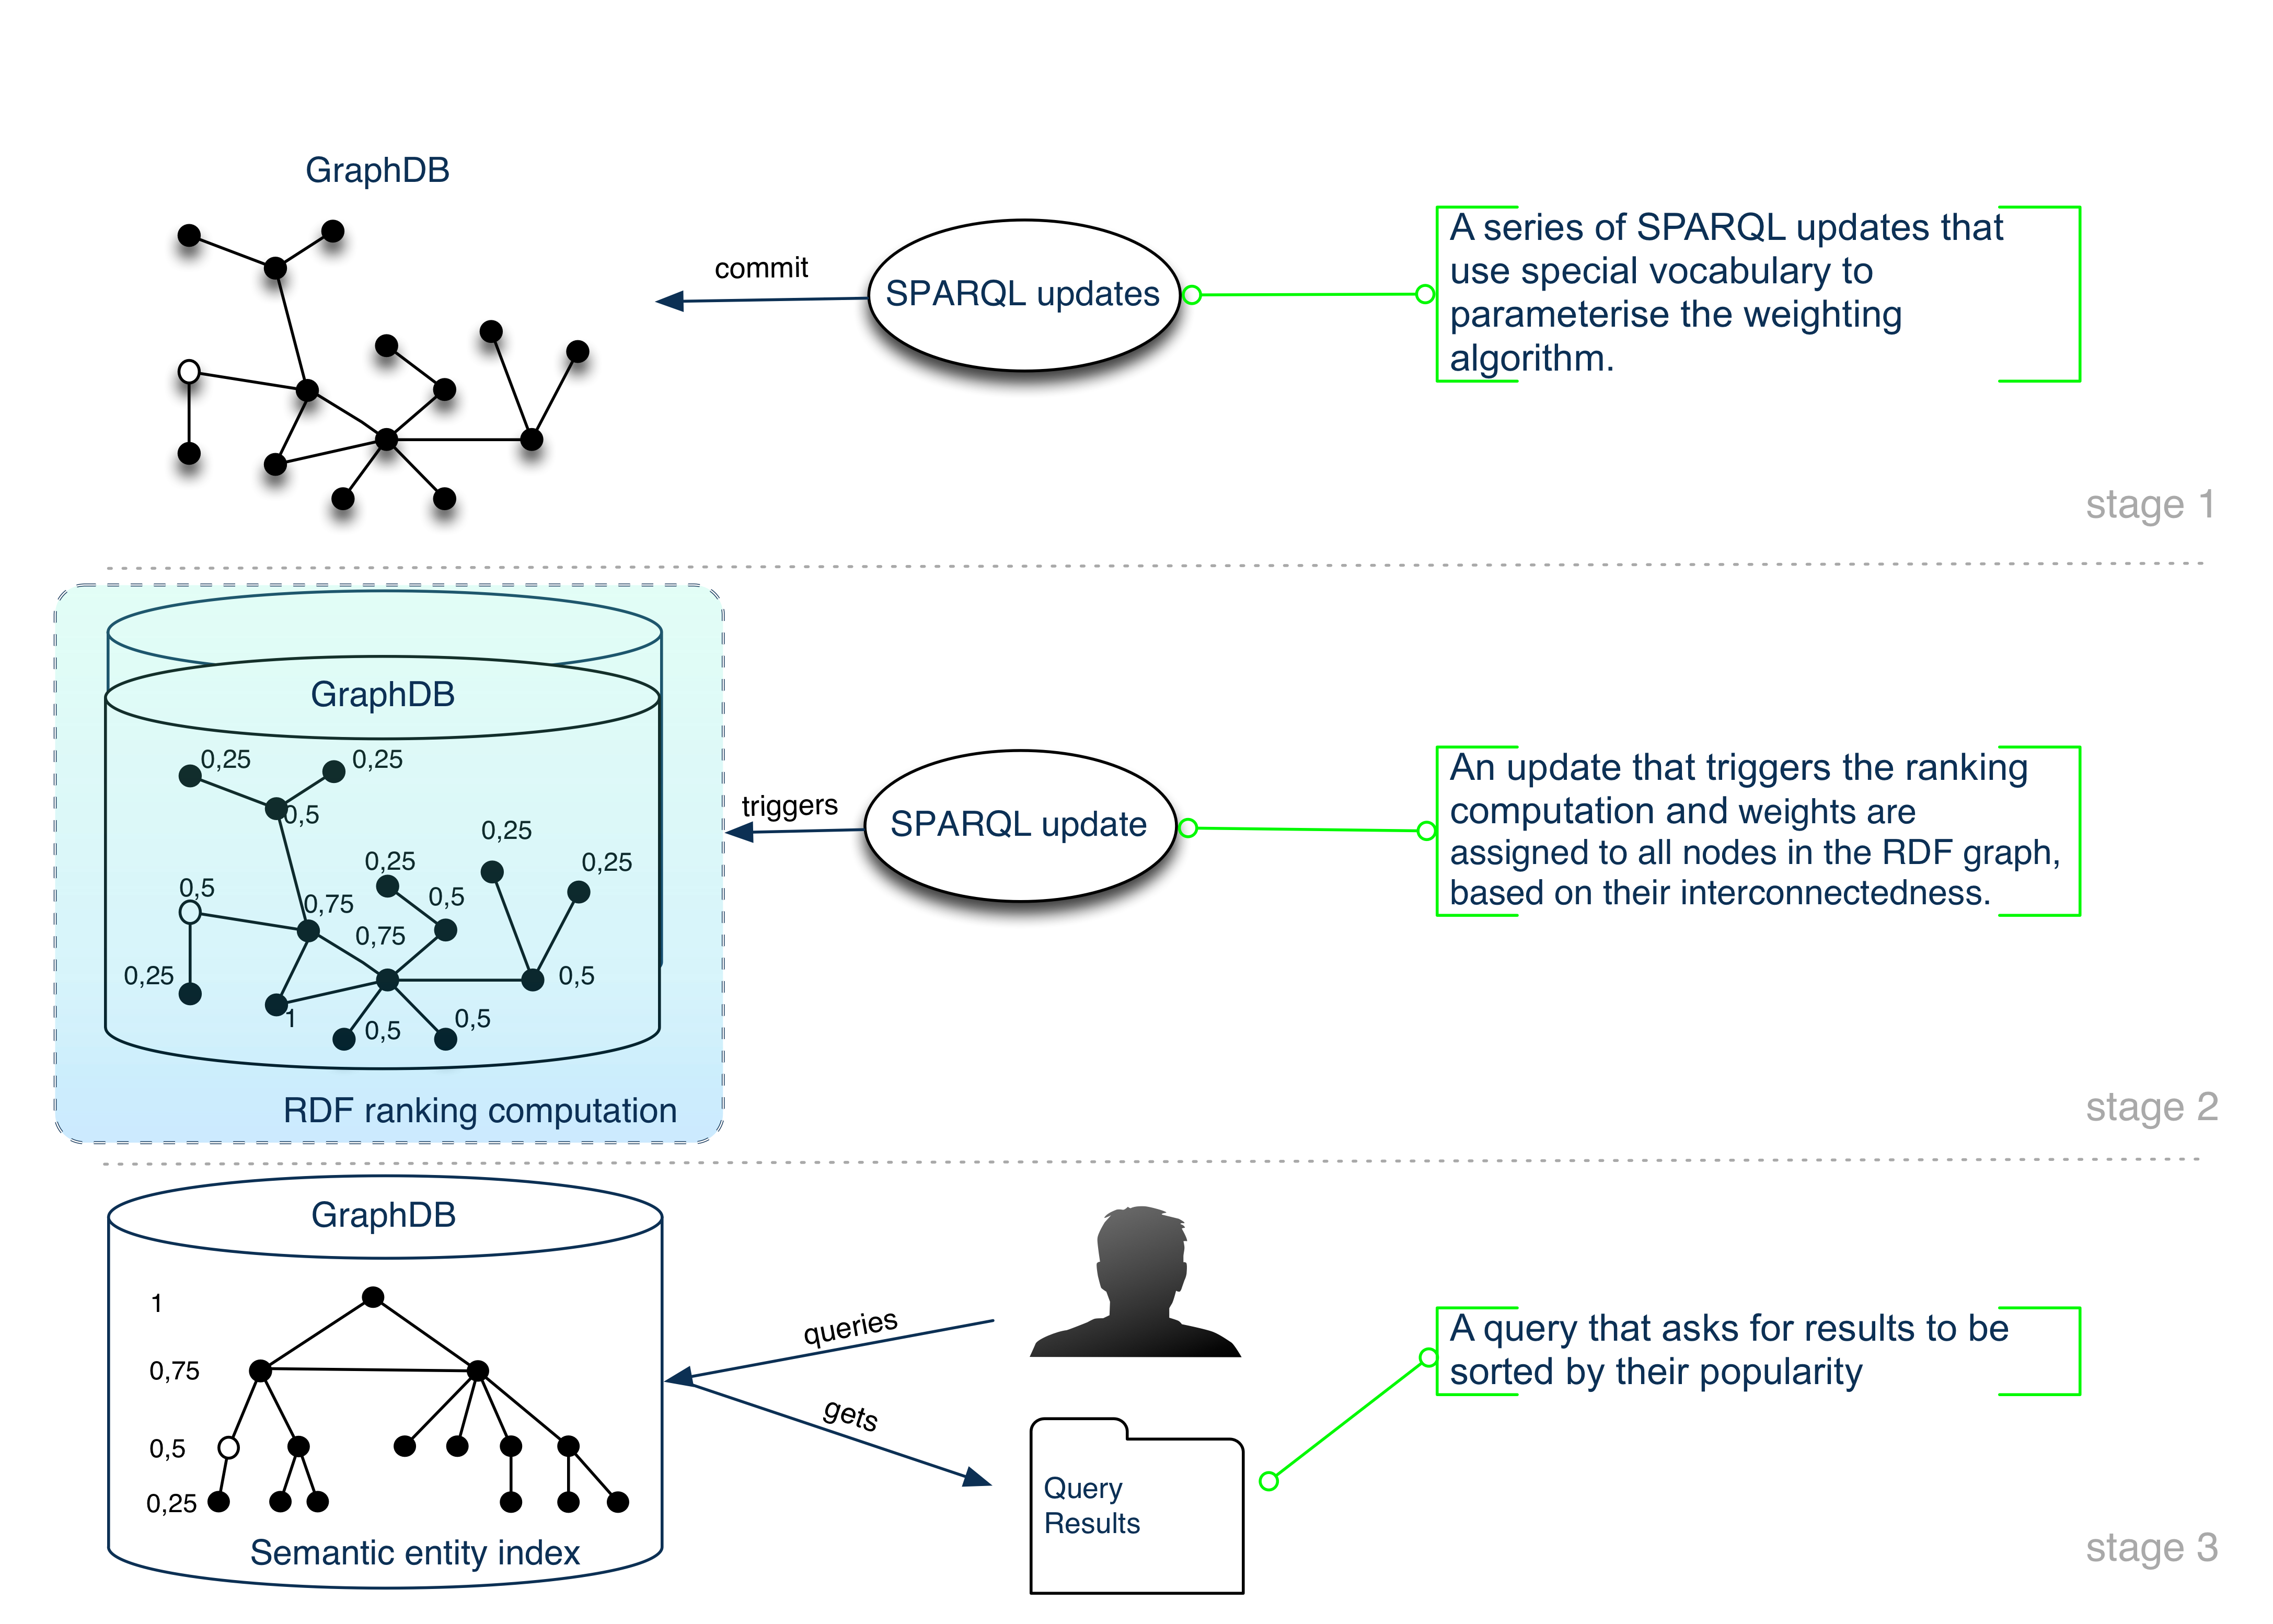
\includegraphics[width=\linewidth]{rdf-rank}
    \caption{RDF Rank plugin workflow}
    \label{rdf-rank}
\end{figure}

\textbf{Context indices} are another optimization that could be utilised, so they will be enabled. There are two types of context indices used to speed up query evaluation when searching statements via their context identifier. These indices are the PCSO (Predicate-Context-Subject-Object) and the PCOS (Predicate-Context-Object-Subject) and they are switched on together.

Finally the \textbf{Lucene Connector} will be used on some key entities from DBPedia and GeoNames and also on news data as a separate index - title, content, creation dates, etc. The Connectors provide synchronisation at the entity level, where an entity is defined as having a unique identifier (a URI) and a set of properties and property values. In terms of RDF, this corresponds to a set of triples that have the same subject. In addition to simple properties (defined by a single triple), the Connectors support property chains. A property chain is defined as a sequence of triples where each triple’s object is the subject of the following triple.

\subsection{FactForge News}
Ontotext has an old free service called \textit{FactForge}, found at \texttt{http://factforge.com}, which is something like a search engine for RDF data. It allows you to write SPARQL queries against these huge amounts of RDF data, e.g. you could ask \textit{"Which are all the airports that in 50km of range of my location?"}. It is basically a triplestore repository with imported and interlinked data sets like GeoNames, DBPedia, etc. and some custom mappings. The setup that has been described so far with our news data in this chapter resembles almost the same thing and eventually it will become exactly that. This huge repository filled with news and popular LOD data sets using the newest version of GraphDB\textsuperscript{TM} and a way more feature-rich and refined Workbench as the user interface, will replace the old FactForge service. It is now called \textit{FactForge News} due to the added news data that was missing in the old one. The next two figures give a small overview of the RDF classes and RDF domain and range relationships of a particular class:

\begin{figure}[h!]
    \centering
    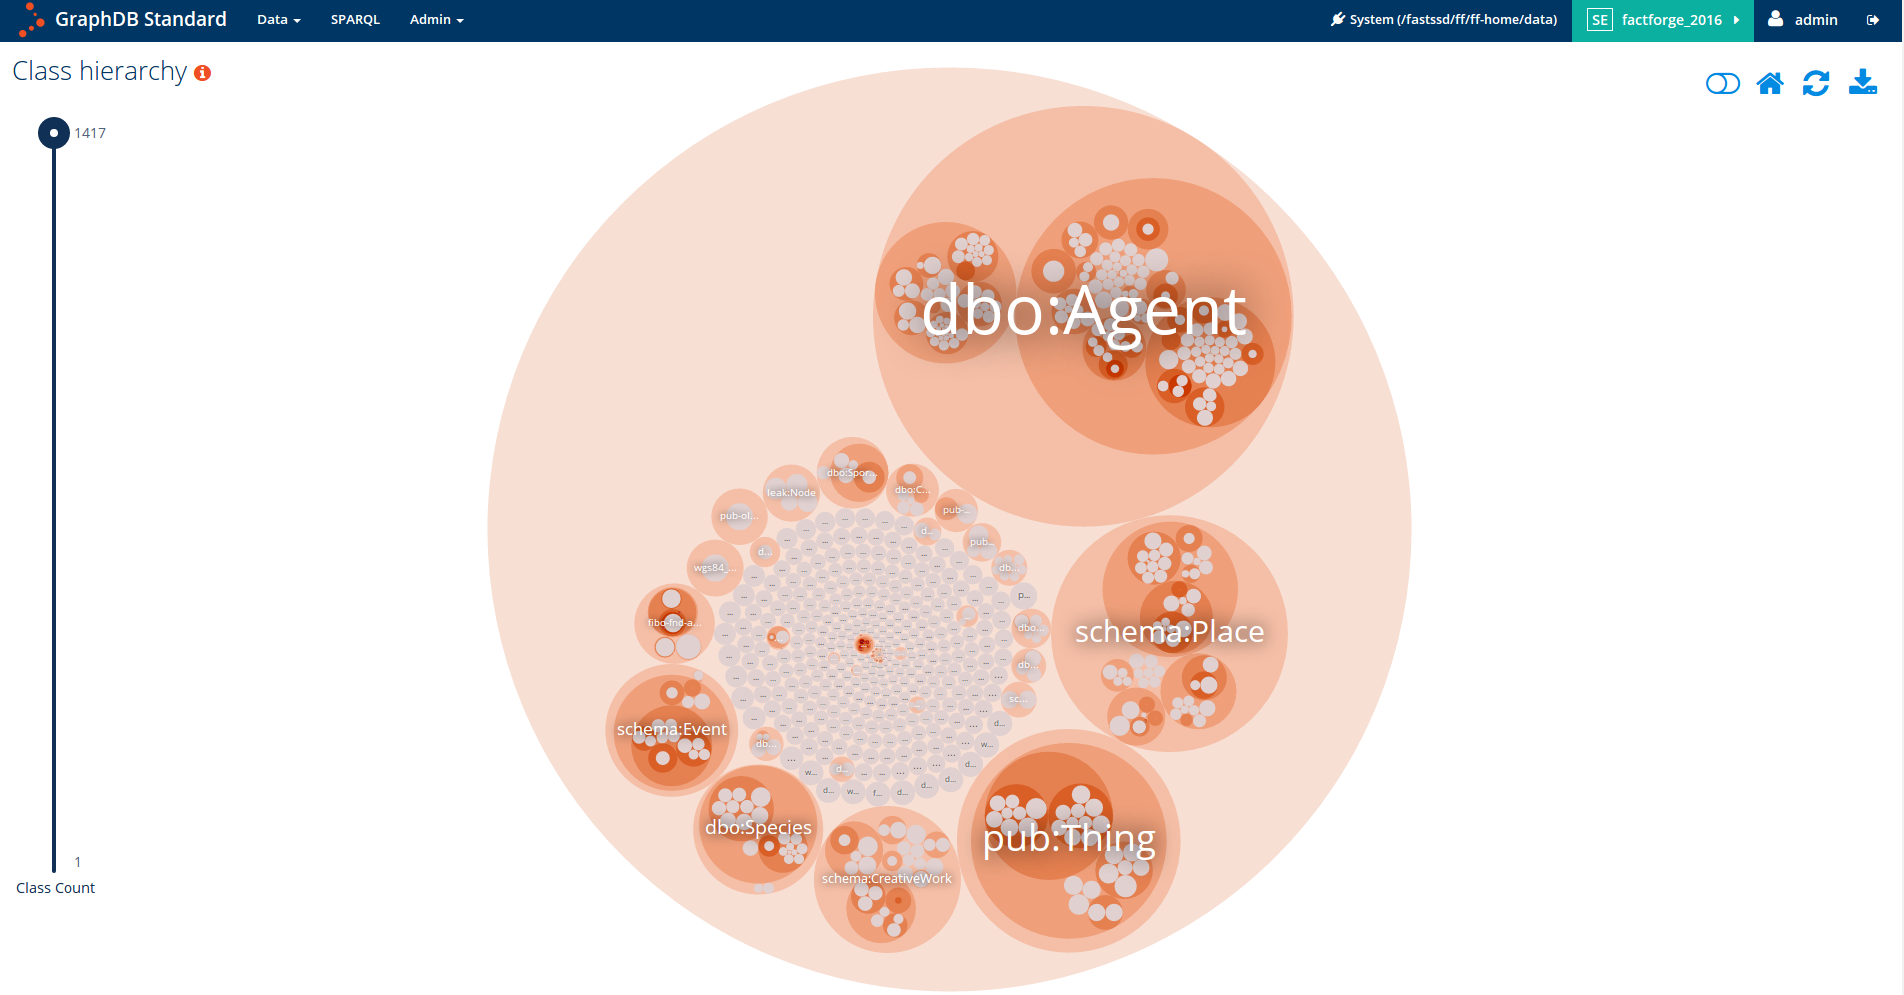
\includegraphics[width=\linewidth]{ff-news-hierarchy}
    \caption{Fact Forge News RDF class hierarchy diagram}
    \label{fig:ff-news-hierarchy}
\end{figure}

\begin{figure}[h!]
    \centering
    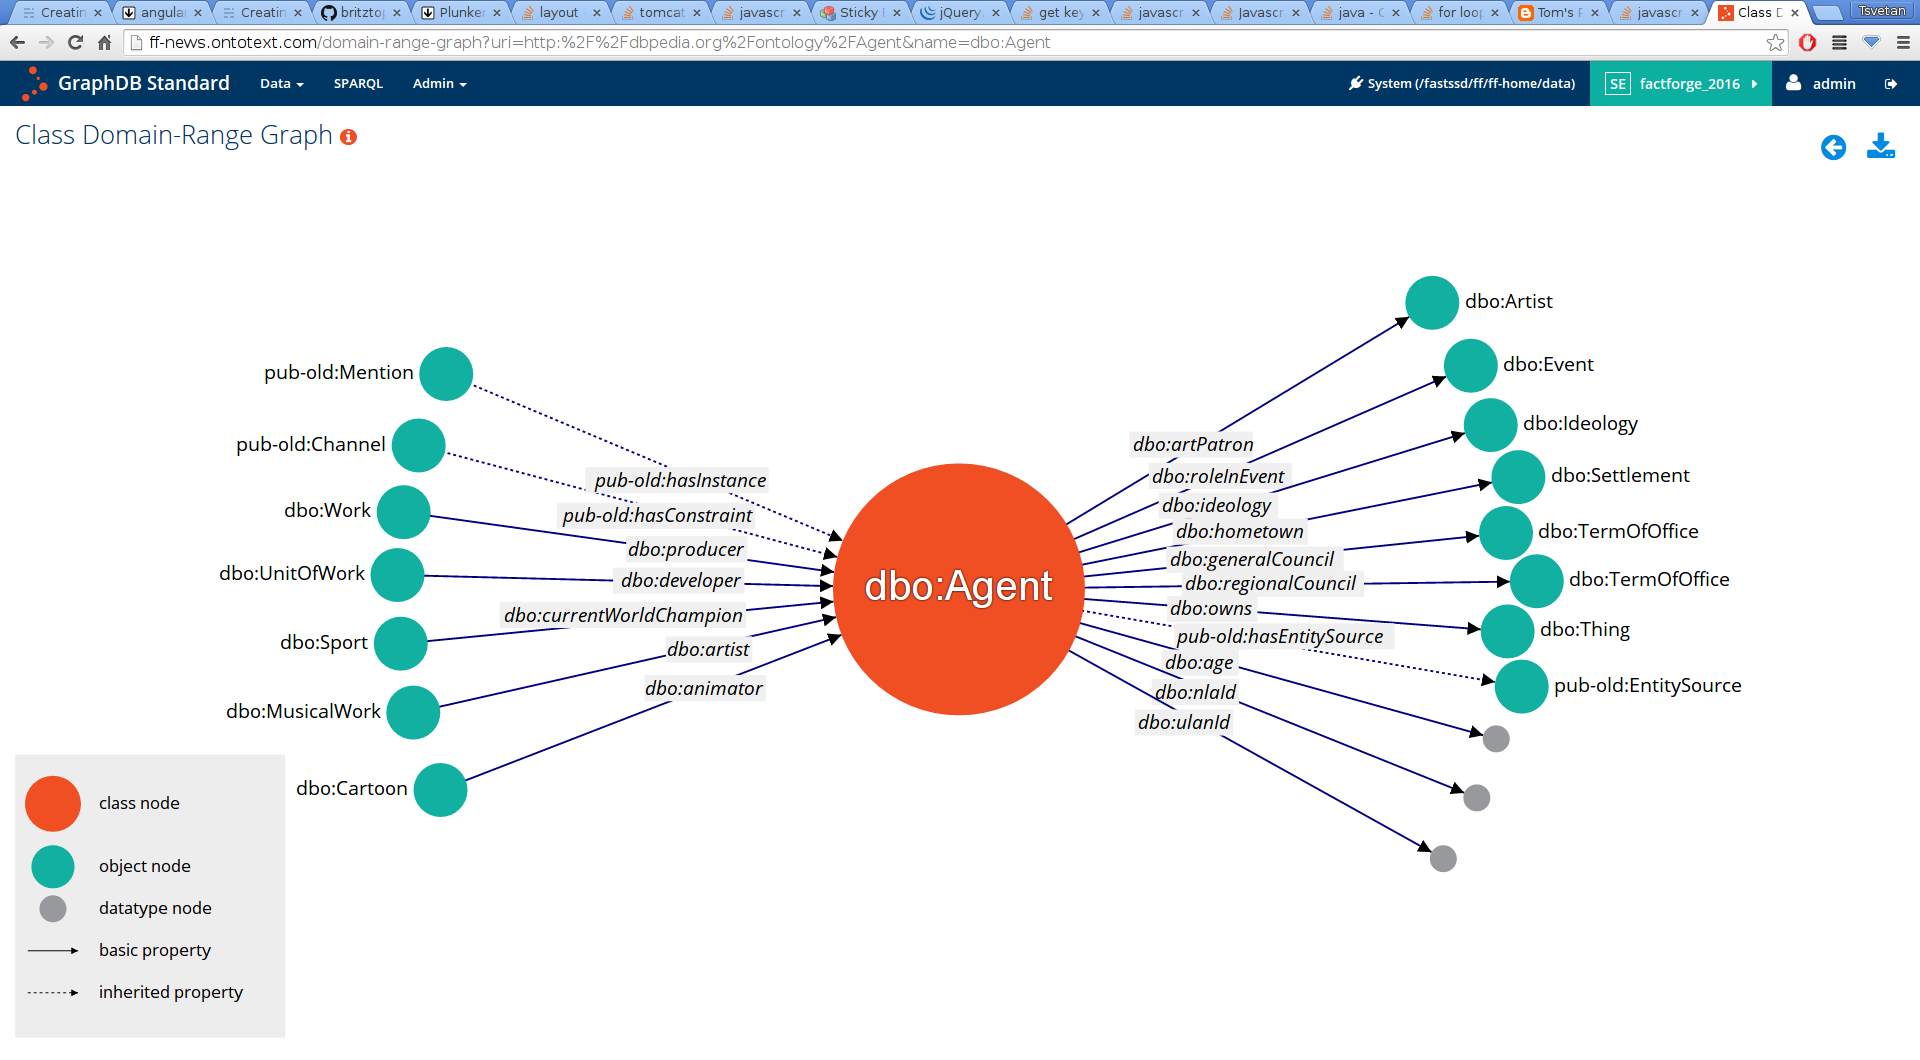
\includegraphics[width=\linewidth]{domain-range-graph-agent}
    \caption{Fact Forge News Agent RDF class domain-range graph diagram}
    \label{fig:domain-range-graph-agent}
\end{figure}
The \textit{Semantic News Map} application presented in \textit{Chapter \ref{chap:semnews-app}} will use \textit{FactForge News} as a data repository. 

\chapter{Semantic News Map Application}
\label{chap:semnews-app}

This chapter will present the end user web application which will visualise the already processed news in various interesting ways. Its goal is to allow you to "read" news in an entirely different way. Usually in articles and almost any other forms of text, the relevant and important information consists in probably less than half the whole text. Harnessing the power of semantics as described in \textit{Chapter \ref{chap:news-pipeline}} with presenting a whole processing pipeline for extracting meaningful information from news data, we now possess an extremely powerful asset extracted in an automated way. The next step is how to present this powerful asset to the user in a unique, effective and interesting way. 

\section{Main Functionalities}
The \textit{Semantic News Map} application consists of a set of visualisations that present the relevant content of a news article or a group of news articles by doing aggregations on the already extracted metadata through SPARQL queries against a GraphDB\textsuperscript{TM} repository with all needed data imported. There are two main types of visualisations: 
\begin{itemize}
    \item Word Cloud
    \item Geographic Heat Map
\end{itemize}
The are a few different versions of word clouds that present data based on different criteria:
\begin{enumerate}
    \item \textbf{Direct popularity} of the concepts based on mentions count in the news and degree of importance of these news.
    \item \textbf{Relative popularity} - where the popularity within the current day is normalized against the popularity within the last year.
    \item Concepts that are \textbf{"hidden champions"} - entities that have an indirect relationship to the currently most popular ones.
    \item Combination of \textbf{"hidden champions"} and \textbf{relative popularity}. 
\end{enumerate}
The geographic heat map has two main functionalities:
\begin{enumerate}
    \item Colors all world countries with different degrees of color intensity according to a specified color scale, based on the number of news in which they are mentioned and displays the news count of each when hovering with the mouse over them.
    \item Presents the list of news mentioning a specific county in a side panel when clicking on it.
\end{enumerate}
\newpage

\begin{figure*}[ht!]
    \centering
    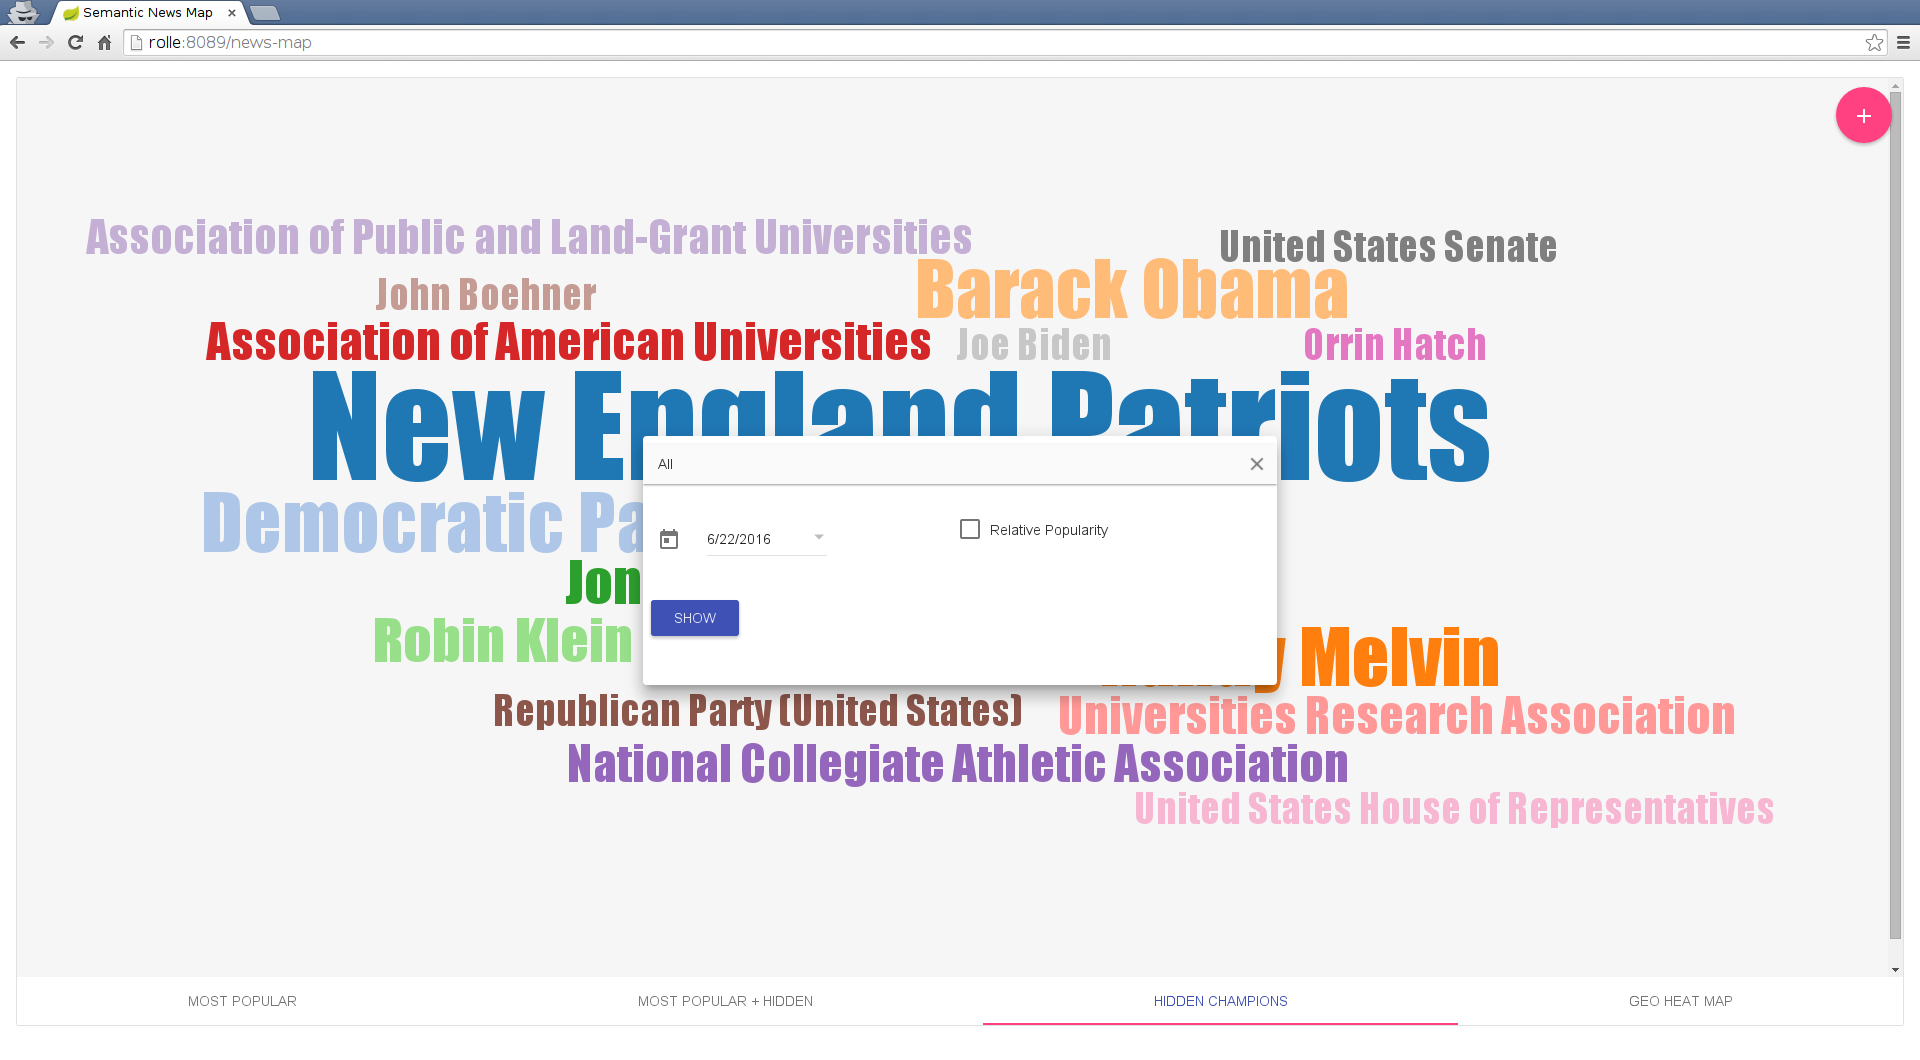
\includegraphics[width=\linewidth]{search-dialog}
    \caption{Hidden Champions criterion word cloud visualisation}
    \label{fig:search-dialog}
\end{figure*}

\begin{figure}[h!]
    \centering
    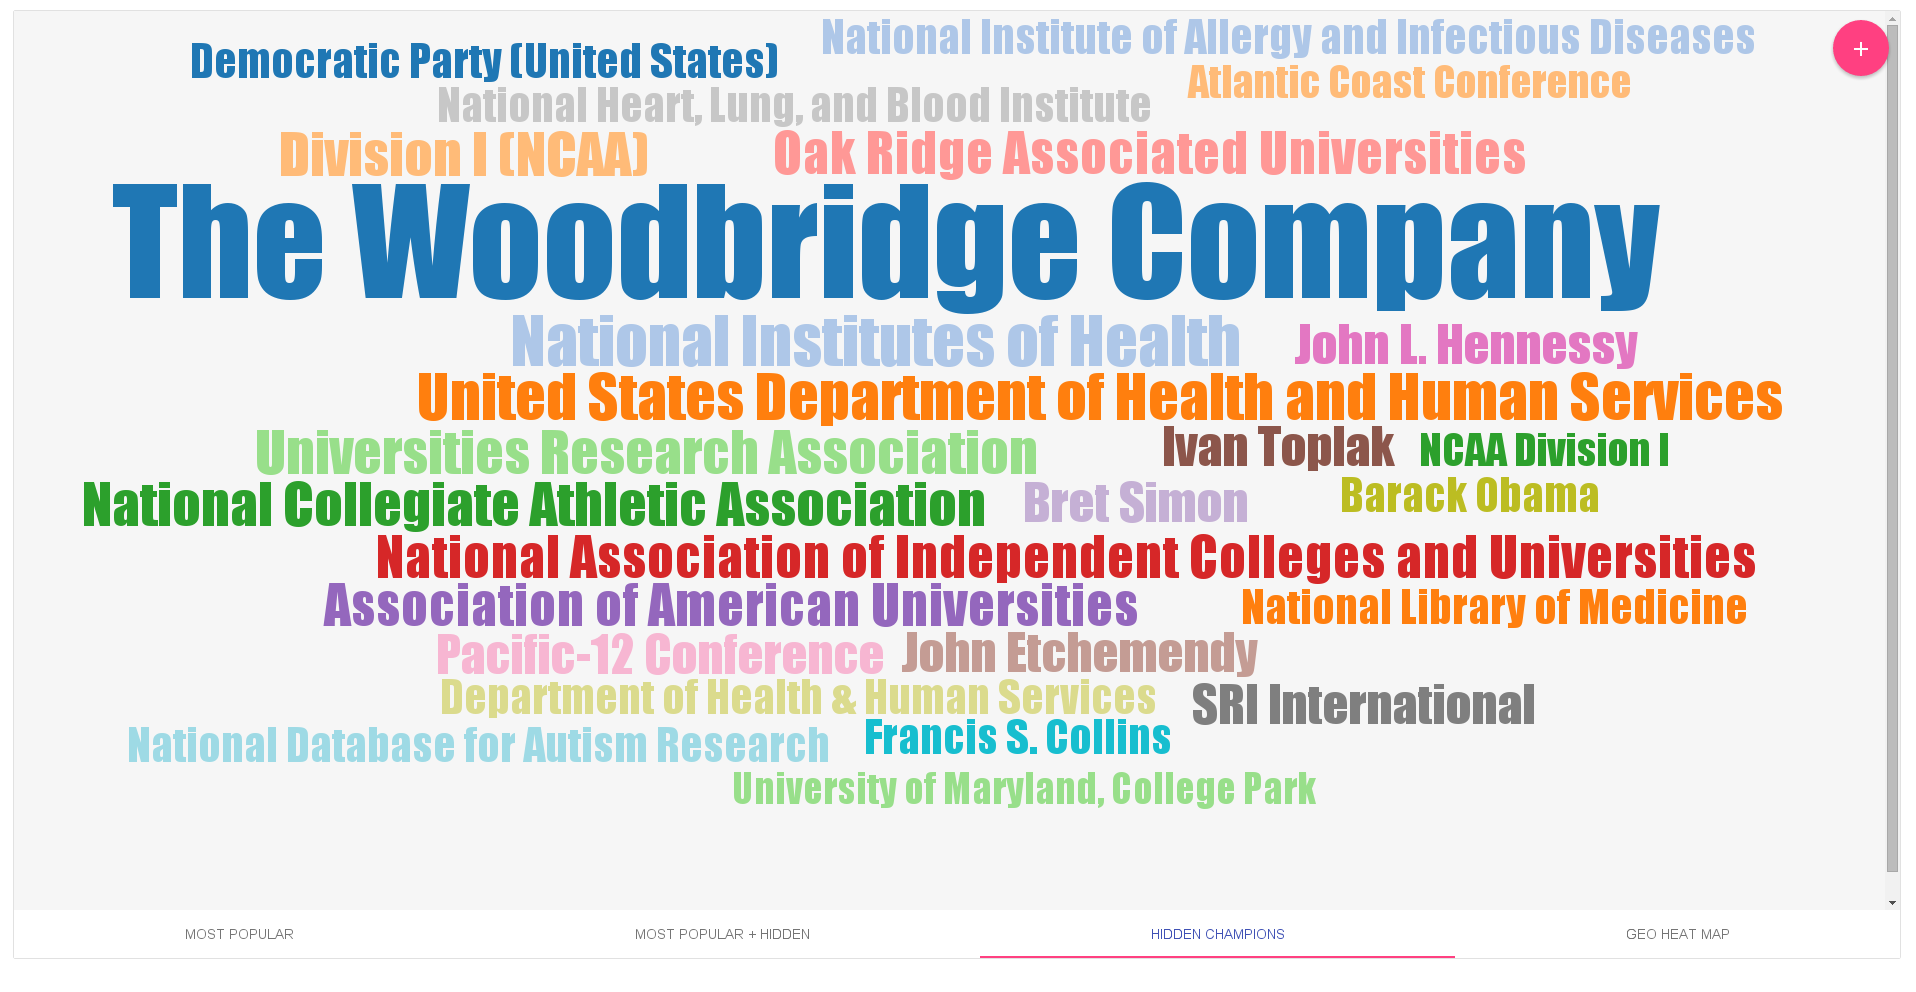
\includegraphics[width=\linewidth]{word-cloud}
    \caption{Hidden Champions criterion word cloud visualisation}
    \label{fig:word-cloud-hidden-champions}
\end{figure}

\begin{figure}[h!]
    \centering
    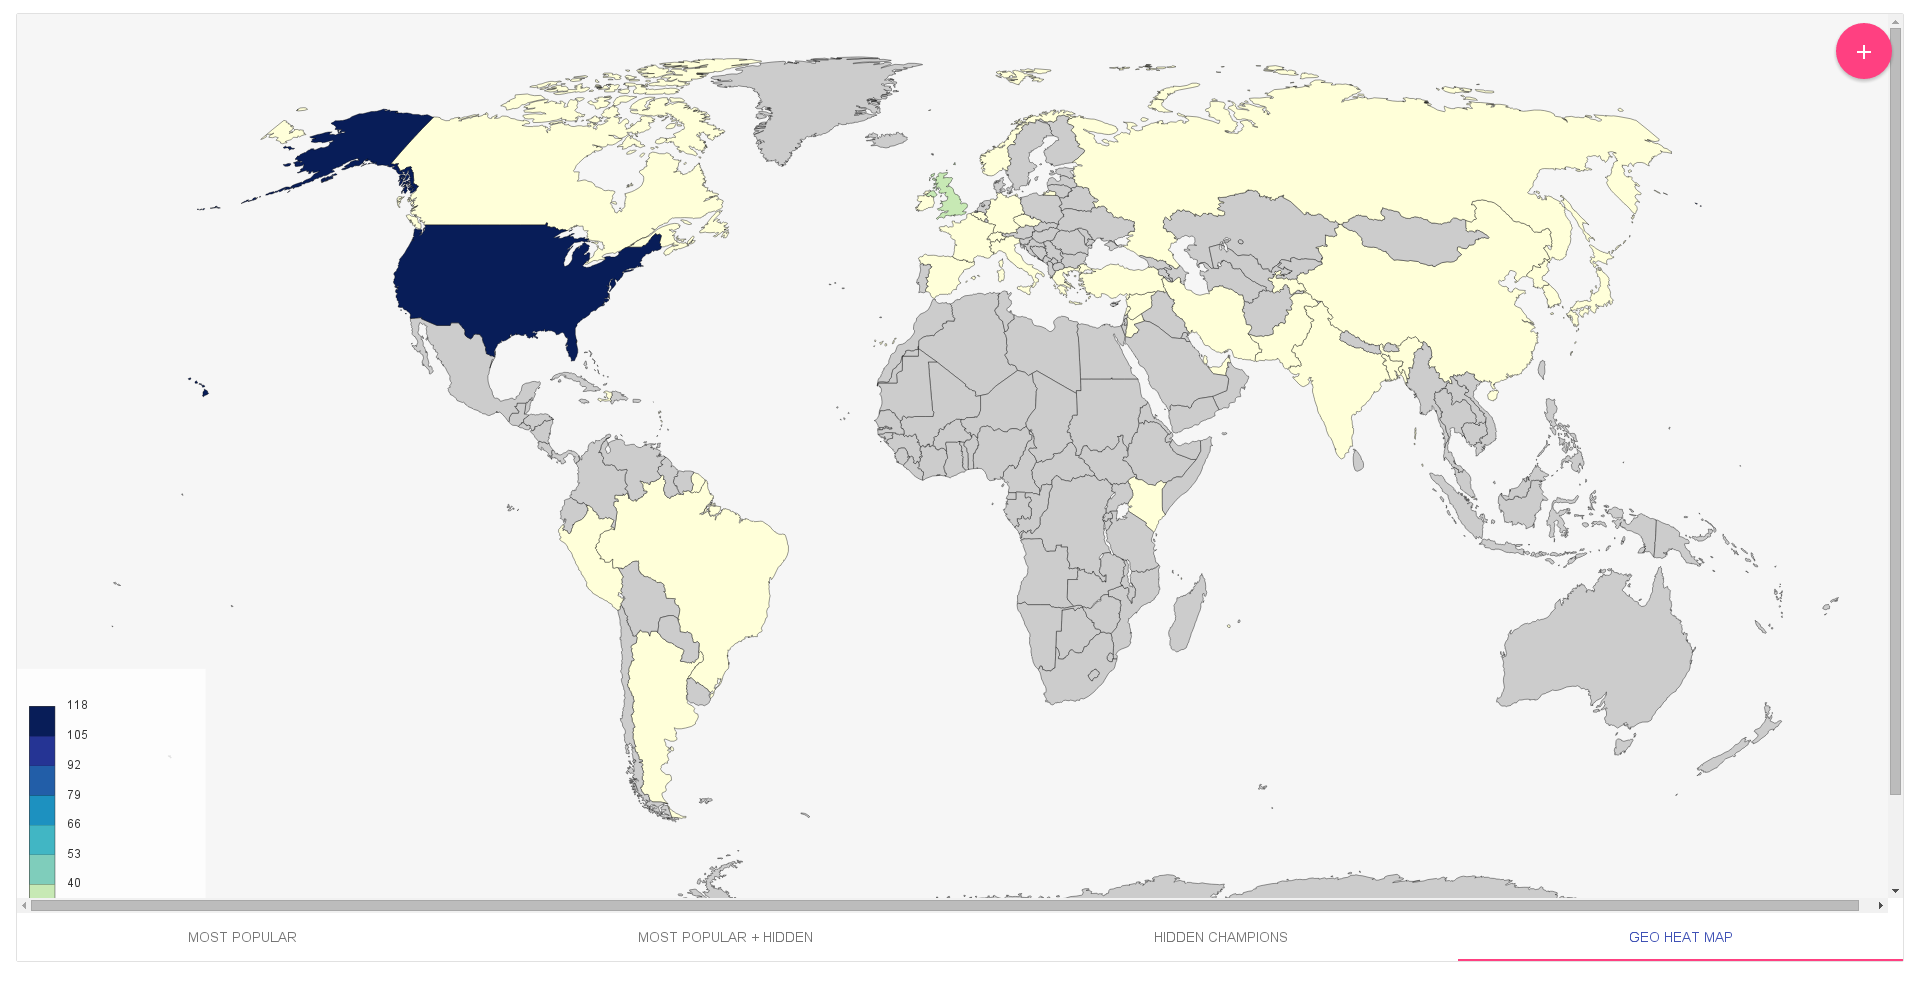
\includegraphics[width=\linewidth]{geoheat-map}
    \caption{Geographic heat map}
    \label{fig:geoheat-map}
\end{figure}

\begin{figure}[h!]
    \centering
    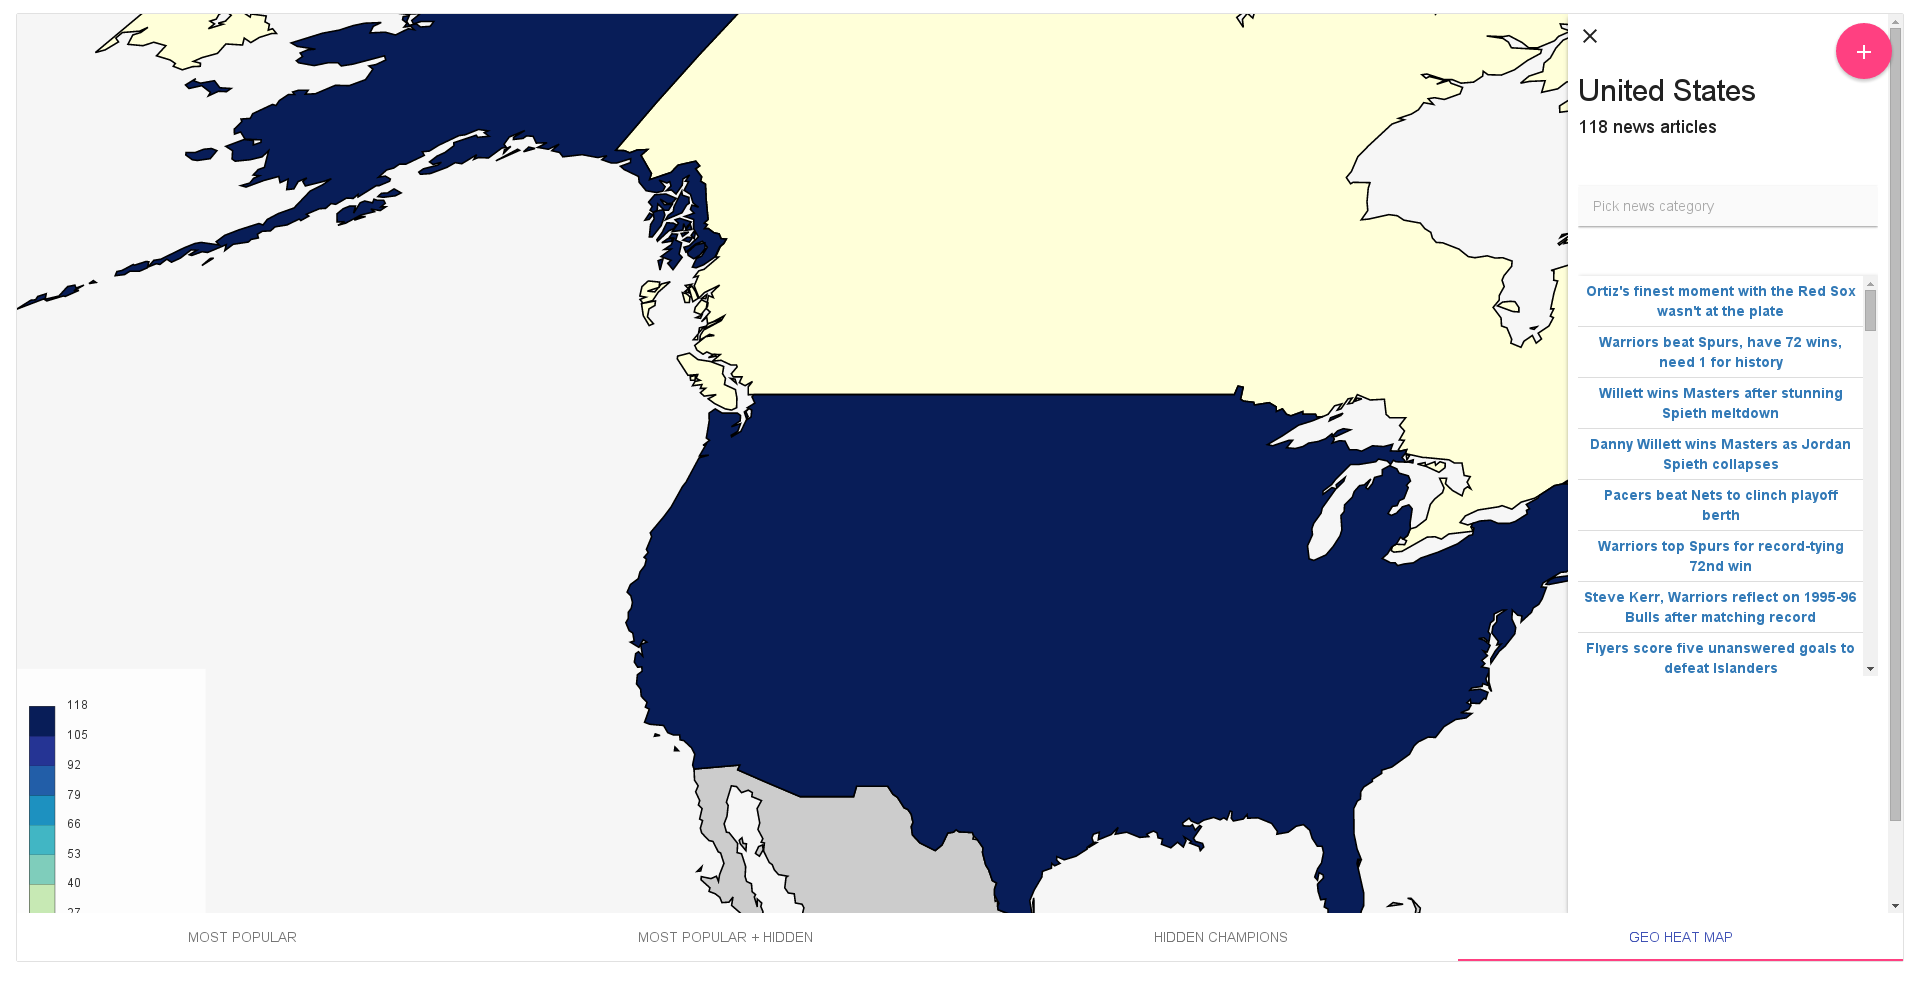
\includegraphics[width=\linewidth]{zoomed-geoheat-map}
    \caption{News mentioning USA and heat map zoomed on USA}
    \label{fig:zoomed-geoheat-map}
\end{figure}

\begin{figure}[h!]
    \centering
    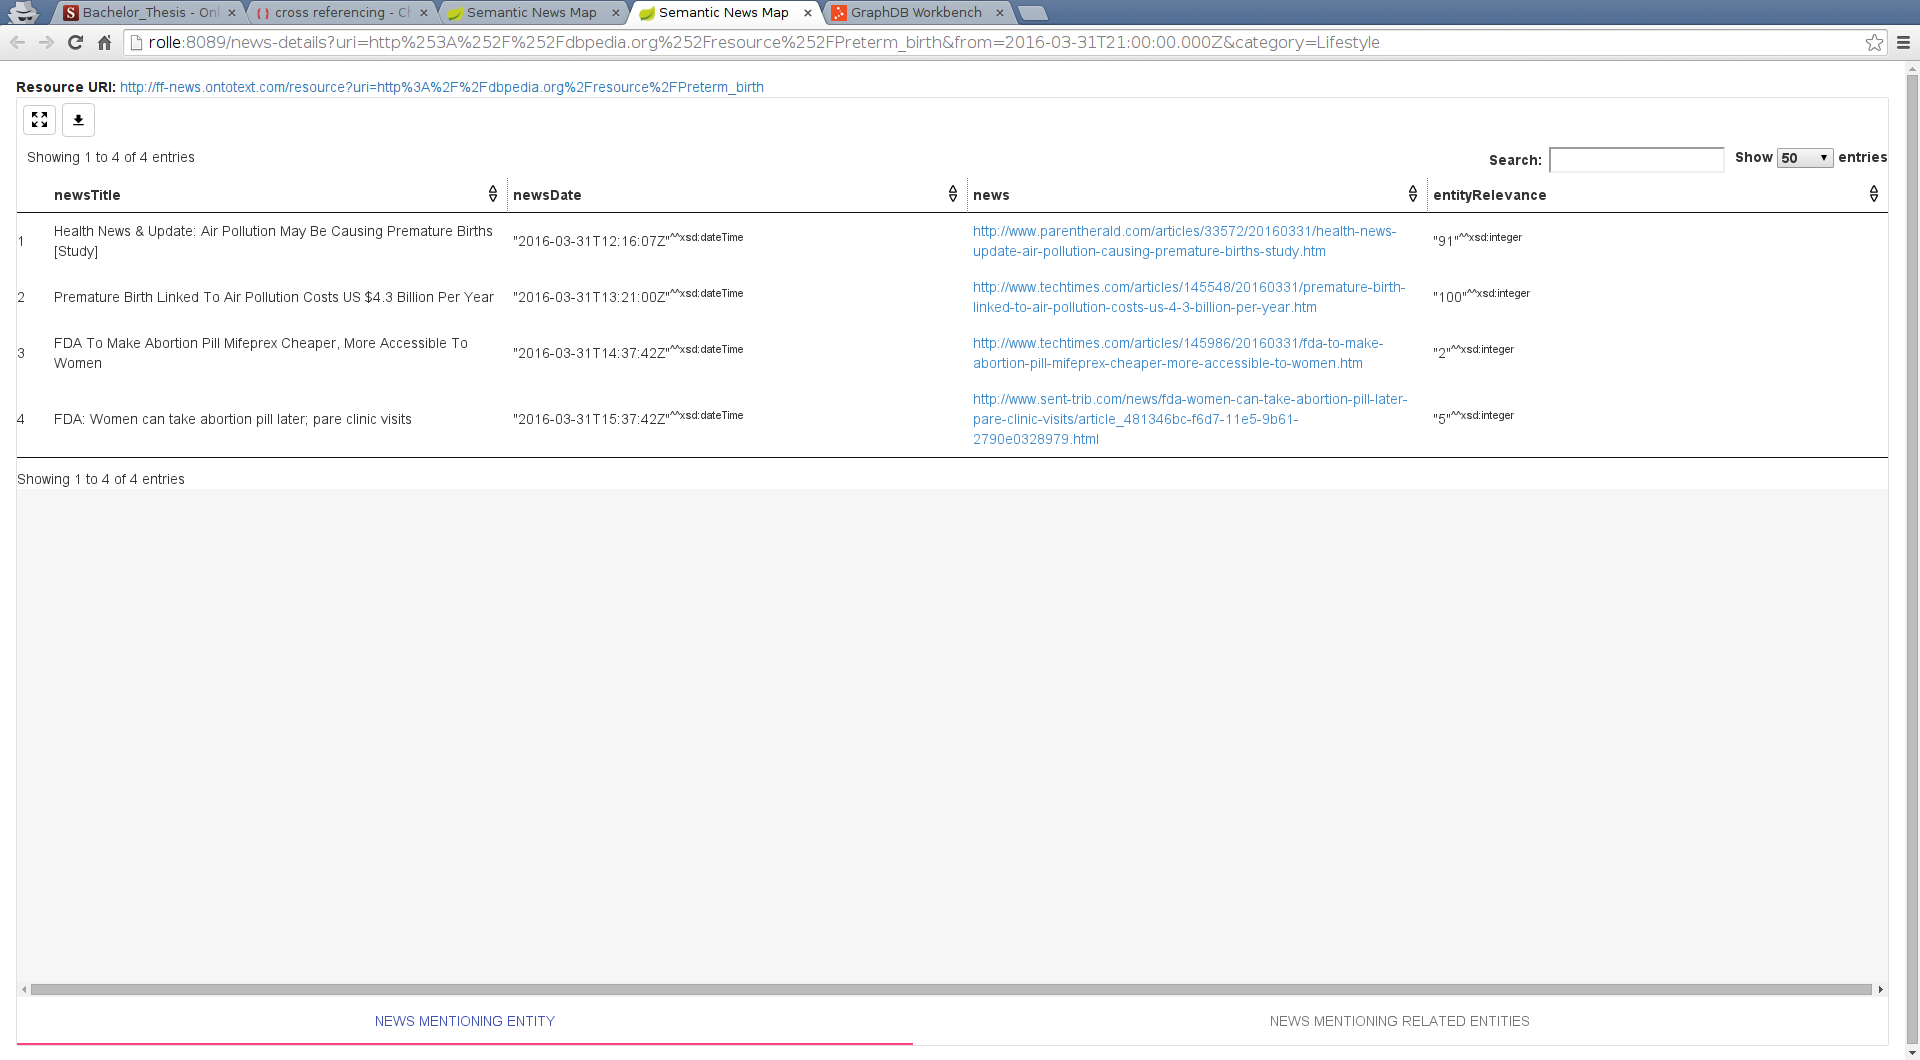
\includegraphics[width=\linewidth]{news-mentioning-entity}
    \caption{News mentioning entity view}
    \label{fig:news-mentioning-entity}
\end{figure}

\begin{figure}[h!]
    \centering
    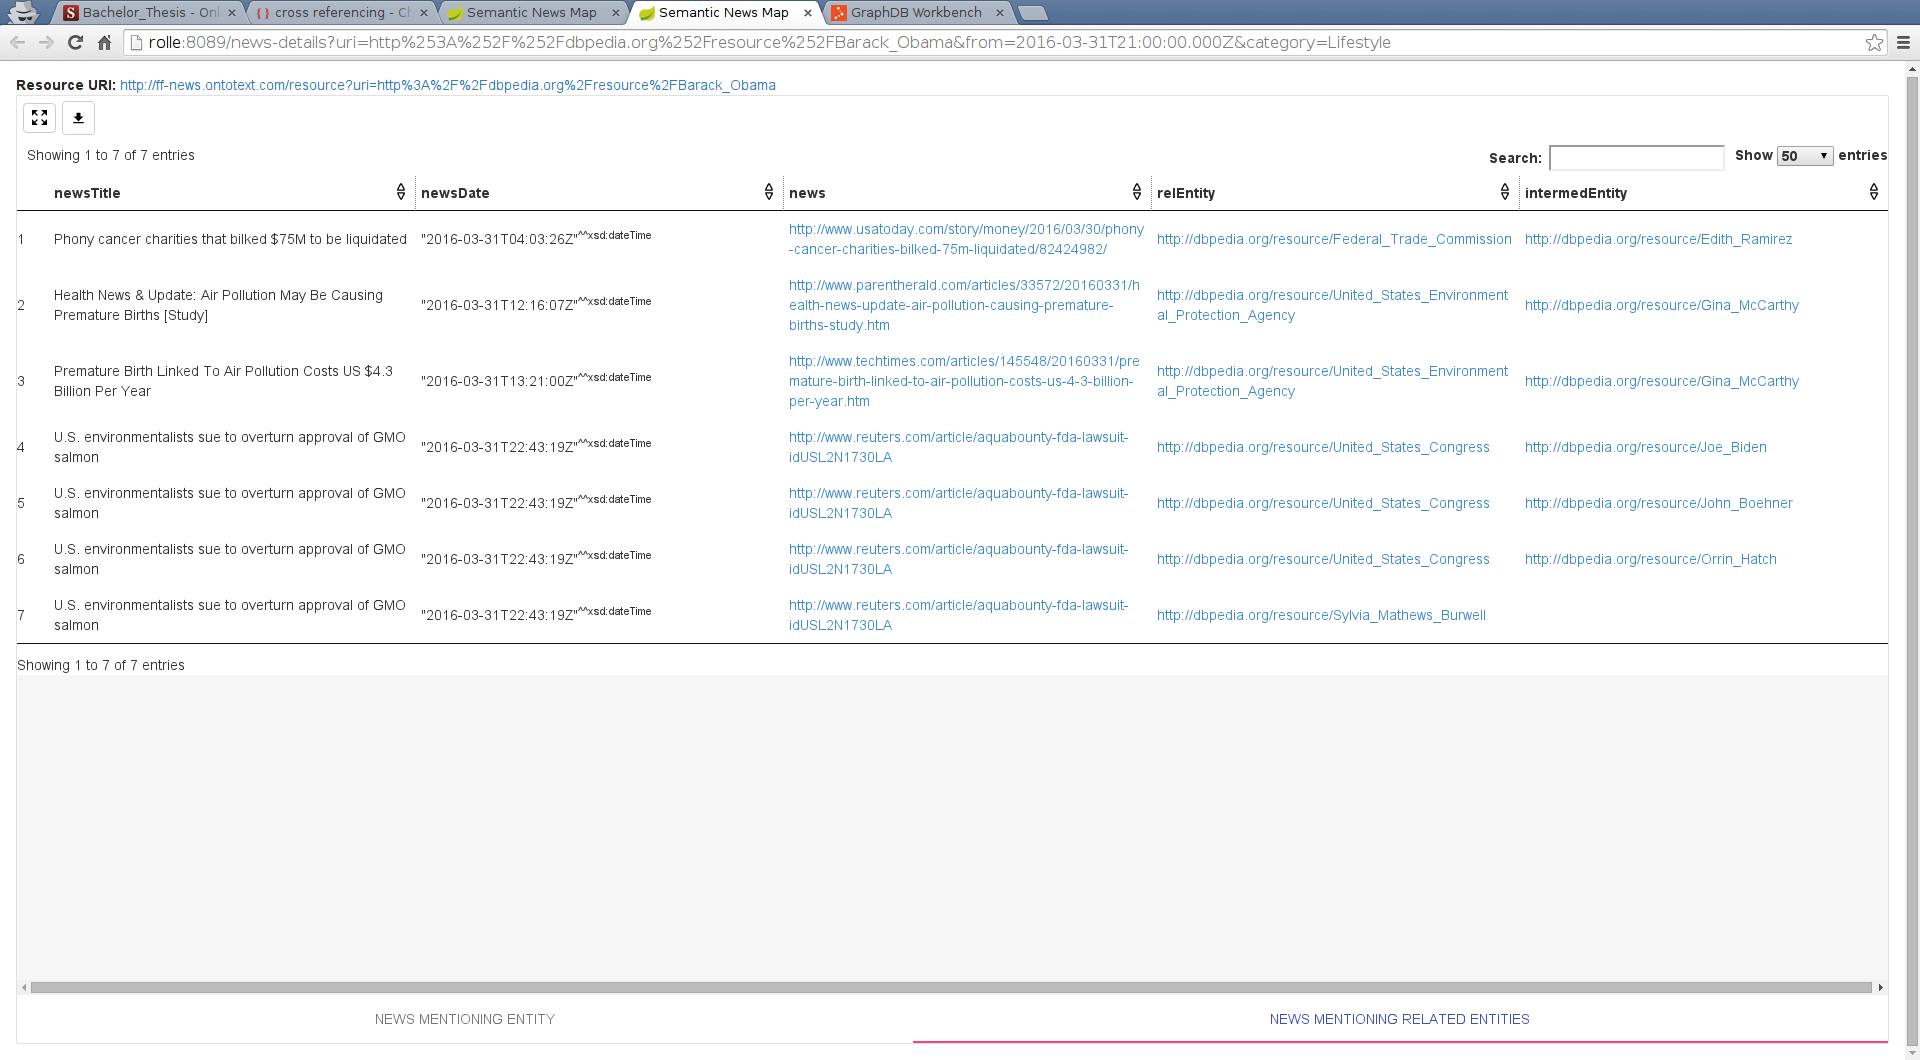
\includegraphics[width=\linewidth]{news-mentioning-related-entities}
    \caption{News mentioning related entities view}
    \label{fig:news-mentioning-related-entities}
\end{figure}



\section{Architecture and used technologies}
The whole application is based on a classic \verb|Client-Server| architecture. There is a backend part and a frontend part. The entire project is managed by \verb|Apache Maven| - a build system for compiling, packaging and dependency management of Java-based projects. It uses the standard Maven project archetype and contains two modules:
\begin{verbatim}
    semantic-news-server
    semantic-news-ui
\end{verbatim}
The first is the backend module which contains only \verb|Java 8| code, connects to the FF-News GraphDB\textsuperscript{TM} repository and executes the news aggregation SPARQL queries which will feed the frontend of the application with data. And the second module is the frontend module which only contains \verb|Javascript|, \verb|HTML| and \verb|CSS| code but its build lifecycle is again managed by Maven.

Communication between both modules is accomplished via REST (Representational State Transfer) in order to assure total decoupling of both components so that they can be easily modified without affecting each other. A simple example could be the frontend making a HTTP request to:\\
\texttt{http://<url-host>/rest/semnews/news-mentioning-country?\\countryCode=USA\&from=2016-04-12}\\ and the backend sending a response containing the results from the execution of the SPARQL query about news titles and URLs of news from 12.April 2016, mentioning the United States in JSON format which the frontend can easily read and handle. 

\subsubsection{Semantic News Map Server (Backend)}
The backend part is written in \texttt{Java 8} using the \texttt{Spring Framework} as a web framework. More specifically \texttt{Spring Boot} is used, which makes it easy to create stand-alone, production-grade Spring based applications that are extremely easy to deploy. It includes an embedded \texttt{Apache Tomcat} application server which eliminates the need for exporting \texttt{.war} files, configuring a Tomcat instance separately, copying the \texttt{.war} file in the Tomcat distribution and launching the server. Spring Boot generates for you an executable \texttt{.jar} file with an already configured embedded application server which only needs to be executed and that is all.

\subsubsection{Semantic News Map UI (Frontend)}
The frontend part is entirely based on AngularJS Javascript MVC framework. AngularJS is a framework for building Single Page Applications (SPA). This means that the server only serves the \texttt{index.html} file on start which then loads all other needed libraries, stylesheets and templates. From there on Angular handles routing, rendering of different views and all other UI specific logic. It will need the backend only as a data provider through AJAX calls to it as was demonstrated above. This style of architecture is called \texttt{Client-Side MVC}.

All Javascript code in the project is written using the newest ECMAScript standard ES6 (ES2015) where there are now features like block-scoped variables with \texttt{let} instead of \texttt{var}, cleaned up syntax for object-oriented programming resembling more Java-style classes and a built-in module system with keywords such as \texttt{import}, \texttt{export} and \texttt{from}. But due to the fact that not all new features are implemented by all browsers, a transpiler called \texttt{Babel} is used which translates code written in ES6 to ES5. The module system at the time of writing this thesis is still not available in any browser yet, so a library called \texttt{SystemJS} is used which expands \texttt{import} statements to SystemJS calls in order to load needed resources.

Javascript dependency management is handled by \texttt{NPM (Node Package Manager)} from NodeJS and \texttt{JSPM}. JSPM is а package manager integrated with SystemJS module loader and works very well with ES6 code.

Most of the UI components are based on Google's design specification \textit{Material Design} used in Android Lollipop and above. AngularJS has an implementation of this spec called \texttt{Angular Material} which is used throughout the whole user interface.

All visualizations in the application are SVG-based and implemented with a library called \texttt{D3 (Data Driven Documents)}. Word clouds use an additional layout to the library called \texttt{d3-cloud} and the geographic heat map also uses an external layout called \texttt{d3-geomap}.

\let\cleardoublepage\clearpage
\chapter{Conclusion}
\section{Analysis}
This thesis has demonstrated how to build an intelligent application based on Semantic Web technologies. News were picked as a use case for this project. They posed the challenge to extract their meaning as being free and unstructured text about any kind of subject or area of life, expressing facts, opinions and conclusions from various different topics and categories. The solution that was presented was based partly on text mining partly on semantic technologies. A semantic news pipeline was presented that included processing steps ranging from raw text entity extraction to conversion to RDF data, interlinked with other Linked Open Data data sets, that enabled writing news aggregation SPARQL queries, against a triplestore repository with the data imported, to really get proper insight about trends of popularity of entities, mentioned in the news.

Finally the results of the news aggregation were presented in the form of SVG-based visualisations as word clouds and geographic heat maps with the user's ability to choose a news category of interest, dates for news published in that period and the option to choose between direct popularity or relative popularity normalized within the last year.

\section{Future directions}
Possible improvements to the \textit{Semantic News Map} could be adding a user base which will keep information about news preferences and also could store rendered visualisations as "Favourites" in your account. News details view could be reworked to be more interactive. More experiments could be done with interesting data sets about, e.g. company information (offshore companies, owners, shareholders, etc.). 

The power of semantics is limitless. It has the unique property to put the world's knowledge under your disposal and actually give you real insight about it. In a world where information is the most valued asset, this technology is priceless. I truly hope that its popularity will continue to grow so that every person on this world could benefit from it.
\appendix
\chapter{Tables}

\clearpage
\newpage

\chapter{Figures}

\clearpage
\newpage

%% This defines the bibliography file (main.bib) and the bibliography style.
%% If you want to create a bibliography file by hand, change the contents of
%% this file to a `thebibliography' environment.  For more information 
%% see section 4.3 of the LaTeX manual.
\begin{singlespace}
\bibliography{main}
\bibliographystyle{plain}
\end{singlespace}

\end{document}

